\documentclass[12pt]{article}

\usepackage{booktabs}% http://ctan.org/pkg/booktabs
\usepackage[utf8]{inputenc}
\usepackage{changepage}
\usepackage{pgfplots}
\usepackage{amssymb}
\usepackage{xcolor}
\usepackage{hyperref}
\usepackage{listings}
\usepackage[T1]{fontenc}
\usepackage[utf8]{inputenc}
\usepackage{adjustbox}
\usepackage{amsmath}
\usepackage{mathtools}
\usepackage{biblatex}
\usepackage{algorithm2e}
\RestyleAlgo{ruled}
\SetKwProg{Proc}{Procedure}{:}{}


\lstset{
  language=Python,
  numbers=left,
  numberstyle=\tiny,
  stepnumber=1,
  numbersep=5pt,
  tabsize=4,
  basicstyle=\ttfamily,
  columns=fullflexible,
  keepspaces,
}
\hypersetup{
    colorlinks,
    citecolor=black,
    filecolor=black,
    linkcolor=black,
    urlcolor=black
}

% Set page size and margins
% Replace `letterpaper' with `a4paper' for UK/EU standard size
\usepackage[letterpaper,top=2cm,bottom=2cm,left=3cm,right=3cm,marginparwidth=1.75cm]{geometry}

% Useful packages
\usepackage{amsmath}
\usepackage{mathtools}
\usepackage{graphicx}
\newenvironment{para}{\begin{adjustwidth}{13mm}{}}{\end{adjustwidth}}

\newcommand\tab[1][1cm]{\hspace*{#1}}

\newcommand{\tabitem}{\llap{\textbullet}}
\newcommand{\Hsquare}{%
\text{\fboxsep=-.2pt\fbox{\rule{0pt}{1ex}\rule{1ex}{0pt}}}%
}

\newtheorem{Definizione}{Definizione}[subsection]
\newtheorem{Lemma}{Lemma}[subsection]
\newtheorem{Teorema/Definizione}{Teorema/Definizione}[subsection]
\newtheorem{Corollario}{Corollario}[subsection]
\newtheorem{Teorema}{Teorema}[subsection]
\newtheorem{Proposizione}{Proposizione}[subsection]
\newtheorem{Notazione}{Notazione}[subsection]
\newtheorem{Commento}{Commento}[subsection]
\newtheorem{Dimostrazione}{Dimostrazione}[subsection]
\newtheorem{Osservazione}{Osservazione}[subsection]
\newtheorem{Nota}{Nota}[subsection]

\DeclarePairedDelimiter\ceil{\lceil}{\rceil}
\DeclarePairedDelimiter\floor{\lfloor}{\rfloor}


\title{Analisi e Progetto di Algoritmi}
\author{spitfire}
\date{A.A. 2024-2025}
\begin{document}
\begin{figure}
    \centering
    
\includegraphics[width=0.35\textwidth]{Images/Logo scienze bicocca.png}
\end{figure}

\vspace{10cm}
\date{A.A. 2024-2025}


\maketitle

\newpage

\tableofcontents
\newpage

\section{Introduzione}
Prima di vedere gli argomenti del corso, facciamo un breve ripasso delle nozioni fondamentali per
lo studio degli algoritmi.
\subsection{Crescita delle funzioni}
Le notazioni che usiamo per descrivere il tempo di esecuzione asintotico di un algoritmo sono definite in termini di funzioni
il cui dominio è l'insieme dei numeri naturali $\mathbb{N} = \{0,1,...\}$. In particolare, indichiamo con:
$$T: \mathbb{N} \rightarrow \mathbb{R}^+$$
la funzione che indica i tempi di calcolo di un algoritmo. Assumiamo che $n$ sia la dimensione dell'input per un certo algoritmo, allora 
$T(n)$ indica il \textbf{tempo di calcolo calcolo (costo computazionale) dell'algoritmo in base alla dimensione dell'input}.
È molto raro avere un espressione ben definita per $T$; infatti molto più spesso interessa maggiormente "come cresce $T$" o più precisamente
\textbf{"$T$ cresce come quale funzione?"}. Siano $g: \mathbb{R} \rightarrow \mathbb{R}^+$ e $f: \mathbb{R}^+ \rightarrow \mathbb{R}^+$ due funzioni (che però applicheremo solo ai naturali).
Diciamo che:
$$\Theta(g(n)) = \left \{f(n)\middle|\exists c_1 >0, c_2 > 0, n_0 \in \mathbb{N}\middle| \forall n \geq n_0, c_1 g(n) \leq f(n) \leq c_2 g(n)\right \}$$
$g(n)$ quindi si dice un \textbf{limite asintotico stretto} per $f$. Una funzione $f(n)$ quindi appartiene a $\Theta(g(n))$ se esistono delle costanti positive $c_1,c_2$ tali che essa possa essere "racchiusa" fra $c_1g(n)$ e $c_2g(n)$ per valori
sufficientemente grandi di $n$. \newline
Se vale solamente che $f(n) \leq c g(n)$ per una qualche costante $c$ allora si dice che $g$ è un \textbf{limite asintotico superiore per $f$} e si indica con $\mathcal{O}(g(n))$. \newline
Se vale solamente che $c g(n) \leq f(n)$ per una qualche costante $c$ allora si dice che $g$ è un \textbf{limite asintotico inferiore per $f$} e si indica con $\Omega(g(n))$. \newline
\begin{center}
    
\includegraphics[width = 1\linewidth]{Images/1.png}
\end{center}
Riportiamo qui di sotto la gerarchia di crescita delle funzioni:
$$\textrm{costante} < \log{n} < n < n \cdot \log n < n^k < 2^n < n! < n^n \; \; \textrm{con } k > 0$$
\subsection{Metodi di risoluzione delle ricorrenze}
Una ricorrenza è un'equazione o disequazione che descrive una funzione
in termini del suo valore con input più piccoli. Vi sono diversi modi per risolvere una ricorrenza:
\begin{itemize}
    \item \textbf{Metodo di sostituzione}: si ipotizza un limite e poi si utilizza l'induzione matematica per dimostrare che l'ipotesi è corretta
    \item \textbf{Metodo dell'albero di ricorsione}: Converte la ricorrenza in un albero i cui nodi rappresentano i costi ai vari livelli della ricorsione.
    \item \textbf{Metodo dell'esperto}: fornice i limiti per le ricorrenze nella forma:
    $$T(n) = aT(\frac{n}{b}) + f(n)$$
    dove $a \geq 1, b>1$ e $f(n)$ è una funzione data. 
\end{itemize}
Possiamo dividere le ricorrenze in due tipi:
\subsubsection{Relazioni di ricorrenza lineari}
\begin{Definizione}
Una relazione di ricorrenza lineare di ordine $r$ è una relazione del tipo:
$$a_n = c_1a_{n-1} + c_2a_{n-2} + ... + c_ra_{n-r} + f(n)$$
dove $c_1, ..., c_r$ sono costanti e $f$ è una funzione di $n$
\end{Definizione}
\begin{Definizione}
    Una relazione di ricorrenza lineare è \textbf{omogenea} di ordine $r$ se è una relazione
    del tipo:
    $$a_n = c_1a_{n-1} + c_2a_{n-2} + ... + c_ra_{n-r}$$
    dove $c_1,...,c_r$ sono costanti
\end{Definizione}
Chiaramente, ogni relazione di ricorrenza lineare omogenea ha la successione identicamente nulla come soluzione.
Analogamente a quanto capita per le equazioni lineari omogenee, si verifica facilmente che combinazioni lineari di soluzioni
di una relazione omogenea sono ancora soluzioni.
\begin{Definizione}
    Diciamo \textbf{polinomio caratteristico} di una relazione di ricorrenza lineare omogenea $R_0$ di ordine $r$ il polinomio:
    $$x^r - c_1x^{r-1} - ... - c_r$$
\end{Definizione}
Vale la seguente proposizione:
\begin{Proposizione}
    Sia $\lambda$ una radice del polinomio caratteristico di una relazione lineare omogenea. Allora la successione $(\lambda^n)_n$ è una soluzione della relazione.
\end{Proposizione}
Vale inoltre, in generale, il seguente teorema:
\begin{Teorema}
    Si consideri una relazione di ricorrenza lineare omogenea di ordine $r$:
    \begin{enumerate}
        \item Supponiamo che la radice $\lambda$ del polinomio caratteristico abbia molteplicità $\mu$. Allora:
        $$\lambda^n, \lambda^n n,\dots,\lambda^n n^{\mu - 1}$$
        sono soluzioni della relazione di ricorrenza. Al variare di $\lambda$ tra le radici del polinomio caratteristico si ottengono $r$ soluzioni di questo tipo, dette le \textbf{soluzioni-base} della relazione.
        \item La soluzione generale della relazione è data da tutte le combinazioni lineari (a coefficienti complessi) delle $r$ soluzioni-base della relazione.
    \end{enumerate}
\end{Teorema}
Analizziamo ora una generica relazione lineare di ordine $r$
$$a_n = c_1a_{n-1} + c_2a_{n-2} + ... + c_ra_{n-r} + f(n)$$
Chiameremo ancora polinomio caratteristico della relazione il polinomio caratteristico della \textbf{relazione omogenea associata}.
\begin{Proposizione}
    La soluzione generale di una relazione di ricorrenza lineare si ottiene aggiungendo una soluzione particolare alla soluzione generale della sua parte omogenea.
\end{Proposizione}
\begin{Proposizione}
    Si consideri una relazione di ricorrenza lineare con parte non omogenea $f$.
    \begin{enumerate}
        \item Sia $f(n) = cq^n$ con $c$ costante e $q \neq 0$. Se $q$ \textbf{non è una radice del polinomio caratteristico}, allora vi è una
        soluzione particolare del tipo $a_n = \alpha q^n$. Se $q$ \textbf{è una radice del polinomio caratteristico di molteplicità} $\mu$, vi è una
        soluzione particolare del tipo $a_n = \alpha n^\mu q^n$. La costante $\alpha$ si determina imponendo che la successione $(a_n)_n$ verifichi la relazione.
        \item Sia $f(n)$ un polinomio in $n$ di grado $k$. Se $1$ \textbf{non è una radice del polinomio caratteristico}, una soluzione particolare è un polinomio di grado $k$ del tipo:
        $$a_n = \alpha_0 + \alpha_1 n + \dots + a_k n^k$$
        Se $1$ \textbf{è una radice del polinomio caratteristico di molteplicità $\mu$}, una soluzione particolare è del tipo $a_n = n^\mu(\alpha_0 + \alpha_1 n + \dots + a_k n^k)$.
        Le costanti $\alpha_0, ..., \alpha_k$ si determinano imponendo che la successione $(a_n)_n$ verifichi la relazione
    \end{enumerate}
\end{Proposizione}
\begin{Corollario}
    Una relazione di ricorrenza lineare il cui termine non omogeneo è costante ammette:
    \begin{itemize}
        \item Una soluzione costante se $1$ \textbf{non è radice del polinomio caratteristico}
        \item Una soluzione del tipo $\alpha n^\mu$ se $1$ è \textbf{radice di molteplicità $\mu$ del polinomio caratteristico}
    \end{itemize}
\end{Corollario}
Una relazione di ricorrenza lineare può essere risolta anche \textbf{osservando che $r^n$ è una soluzione per particolari valori di $r$}.
Per relazioni di ricorrenza della forma:
$$x_n = Ax_{n-1} + Bx_{n-2}$$
si ha la soluzione $r^n$ per la quale:
$$r^n = Ar^{n-1} + Br^{n-2}$$
dividendo tutti i termini per $r^{n-2}$ si ottiene:
$$r^2 = Ar + B$$
ossia
$$r^2 - Ar - B = 0$$
che viene chiamata \textbf{equazione caratteristica della relazione di ricorrenza}. Essa fornisce per $r$ due radici
$\lambda_1, \lambda_2$. Se tali radici sono \textbf{distinte} si ha la soluzione:
$$x_n = C\lambda_1^n + D\lambda_2^n$$
se invece le due radici \textbf{coincidono}, cioè se $A^2 +4B = 0$ si ha:
$$x_n = C\lambda^n + Dn\lambda^n$$
dove $C$ e $D$ sono costanti arbitrarie che possono essere ricavate da "condizioni al contorno" che tipicamente
sono date nella forma:
$$x_0 = a, \; \; x_1 = b$$
\subsubsection{Metodo di sostituzione}
Il metodo di \textbf{sostituzione} per risolvere le ricorrenze richiede due passi:
\begin{enumerate}
    \item Ipotizzare la forma della soluzione
    \item Usare l'induzione matematica per trovare le costanti e dimostrare che la soluzione funziona
\end{enumerate}
Il nome del metodo deriva dalla sostituzione della soluzione ipotizzata al posto della funzione quando l'ipotesi induttiva viene
applicata a valori più piccoli. Questo metodo è potente, ma ovviamente può essere applicato solamente a ricorrenze di cui
sia facile immaginare la forma della soluzione. Inoltre, non esiste un metodo generale per effettuare una buona ipotesi, quindi bisogna
basarsi molto spesso sull'esperienza oppure controllare se la ricorrenza considerata è simile a ricorrenze di cui si conoscono già i limiti
asintotici. Altri metodi per risolvere le problematiche di questo metodo sono:
\begin{itemize}
    \item \textbf{Effettuare ipotesi "lasche"} e man mano diminuire il grado di incertezza (cioè, restringere le ipotesi fino ad arrivare ad un limite stretto)
    \item \textbf{Sottrarre un termine di grado inferiore}, sopratutto in ricorrenze in cui l'ipotesi induttiva non è abbastanza forte per dimostrare il limite esatto per colpa di una costante
    \item \textbf{Sostituzioni di variabili}
\end{itemize}
\subsubsection{Metodo dell'albero di ricorsione}
In un \textbf{albero di ricorsione}, ogni nodo rappresenta il costo di un \textbf{singolo sotto-problema} da qualche parte nell'insieme
delle chiamate ricorsive di funzione. Sommiamo i costi all'interno di ogni livello dell'albero per ottenere un insieme di costi per livello;
poi sommiamo tutti i costi per livello per determinare il costo totale di tutti i livelli della ricorsione.
Un albero di ricorsione è un ottimo modo per \textbf{ottenere una buona ipotesi} che verrà poi verificata tramite il \textbf{metodo di sostituzione}; tuttavia
può essere usato anche come metodo risolutivo diretto.
\begin{center}
    
\includegraphics[width = 1\linewidth]{Images/2.png}
\end{center}
\begin{center}
    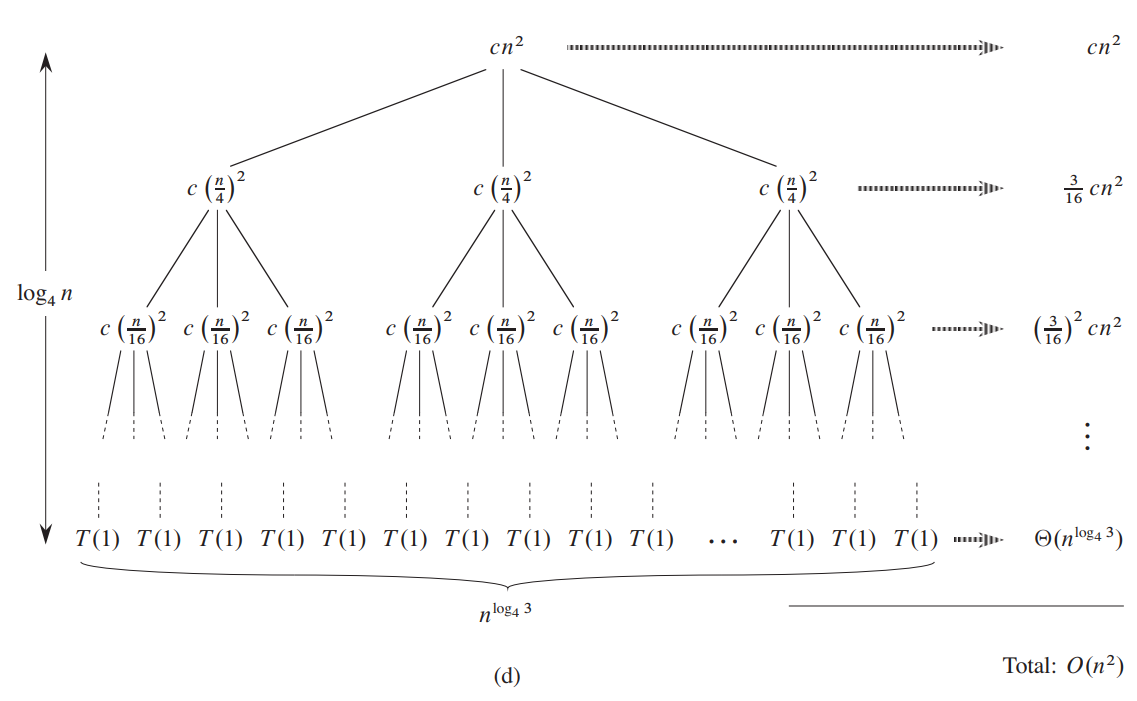
\includegraphics[width = 1\linewidth]{Images/3.png}
\end{center}
\subsubsection{Metodo dell'esperto}
Il metodo dell'esperto permette di risolvere le ricorrenze della forma:
$$T(n) = aT(\frac{n}{b}) + f(n)$$
dove $a \geq 1, b >1$ sono costanti e $f(n)$ è una funzione \textbf{asintoticamente positiva}.
Il metodo dell'esperto dipende dal seguente teorema:
\begin{Teorema}[Teorema dell'esperto]
    Date le costanti $a \geq 1, b > 1$ e la funzione $f(n)$, sia $T(n)$ una funzione definita sugli interi non negativi dalla ricorrenza
    $$T(n) = aT(\frac{n}{b}) + f(n)$$
    dove $\frac{n}{b}$ rappresenta $\floor{\frac{n}{b}}$ o $\ceil{\frac{n}{b}}$. Allora $T(n)$ può essere asintoticamente limitata nei seguenti modi:
    \begin{enumerate}
        \item Se $f(n) = \mathcal{O}(n^{\log_b{a - \varepsilon}})$ per qualche costante $\varepsilon > 0$, allora $T(n) = \Theta(n^{lob_b{a}})$
        \item Se $f(n) = \Theta(n^{\log_b{a}})$ allora $T(n) = \Theta(n^{\log_b{a}} \log{n})$
        \item Se $f(n) = \Omega(n^{log_b{a} + \varepsilon})$ per qualche costante $\varepsilon > 0$ e se $f(\frac{n}{b}) \leq c f(n)$ per qualche costante $c < 1$ e per ogni
        $n$ sufficientemente grande, allora $T(n) = \Theta(f(n))$
    \end{enumerate}
\end{Teorema}
Questo metodo si utilizza principalmente per risolvere le ricorrenze che descrivono i tempi di calcolo degli algoritmi
\textbf{dividi-et-impera}
\section{Programmazione dinamica}
La programmazione dinamica risolve i problemi combinando le soluzioni dei sotto-problemi.
La tecnica dividi-et-impera, divide il problema in sotto-problemi \textbf{indipendenti}, li risolve in modo ricorsivo e, poi, combina
le loro soluzioni per risolvere il problema originale. La programmazione dinamica, invece, può essere applicata quando \textbf{i sotto-problemi non sono indipendenti},
ovvero quando i sotto-problemi hanno \textbf{in comune dei sotto-problemi}. In questo contesto, un algoritmo dividi-et-impera \textbf{svolge molto più lavoro del necessario},
risolvendo \textbf{ripetutamente i sotto-problemi comuni}. Un algoritmo di programmazione dinamica invece \textbf{calcola una sola volta i risultati dei sotto-problemi} e li
salva in una tabella, evitando quindi di ricalcolarli ogni volta che essi si presentano. La programmazione dinamica tendenzialmente si applica ai \textbf{problemi di ottimizzazione}.
Per questi problemi ci possono essere molte soluzioni possibili; quindi si vuole trovare una soluzione con \textbf{valore ottimo} (minimo o massimo). Precisiamo che abbiamo detto \textbf{UNA} soluzione
ottima e non \textbf{LA} soluzione ottima poiché ci possono essere più soluzioni che raggiungono il valore ottimo.
Il processo di sviluppo di un algoritmo di programmazione dinamica può essere suddiviso in una sequenza di quattro fasi:
\begin{enumerate}
    \item Caratterizzare la struttura di una soluzione ottima
    \item Definire in modo ricorsivo il valore di una soluzione ottima
    \item Calcolare il valore di una soluzione ottima, di solito con uno schema bottom-up (dal basso verso l'alto)
    \item Costruire una soluzione ottima dalle informazione calcolate (algoritmo di \textbf{ricostruzione})
\end{enumerate}
Durante la fase 4 possiamo memorizzare anche \textbf{informazioni aggiuntive} utili a semplificare il processo di ricostruzione.
Facciamo un esempio: consideriamo un algoritmo ricorsivo che dia in output l'n-esimo numero di fibonacci: \newline
\begin{algorithm}[H]
\caption{Algoritmo ricorsivo che calcola l'n-esimo numero di fibonacci}
\DontPrintSemicolon
\SetKwFunction{FFibRic}{Fib-Ric}
\Proc{\FFibRic{n}} {
    \eIf{n $\leq$ 1} {
        \Return 1
    } {
        \Return Fib-Ric(n-1) + Fib-Ric(n-2)
    }
}
\end{algorithm}
\noindent
La sua equazione di ricorrenza è:
$$T(n) = T(n-1) + T(n-2) + 2$$
Se provassi a sviluppare la ricorrenza, finirei in un \textbf{loop infinito}. 
Proviamo quindi il metodo dell'albero di ricorsione; supponiamo $n = 5$:
\begin{center}
    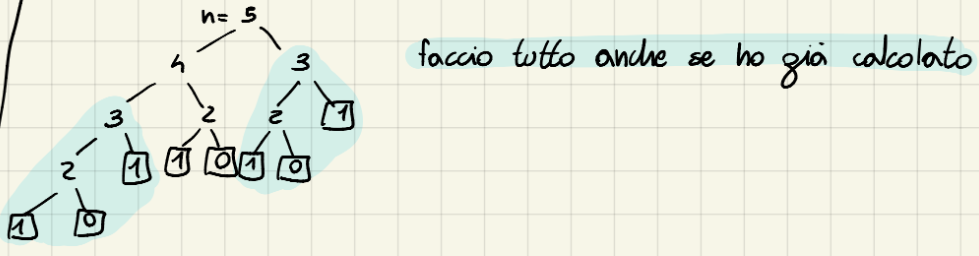
\includegraphics[width = 1\linewidth]{Images/4.png}
\end{center}
notiamo quindi che l'algoritmo \textbf{non si accorge che alcuni calcoli si ripetono}. Notiamo quindi
che l'equazione di ricorrenza è una \textbf{ricorrenza lineare non omogenea}; consideriamo quindi l'equazione
di ricorrenza omogenea associata:
$$T(n) = T(n-1) + T(n-2)$$
supponiamo che $r^n$ è una soluzione:
$$r^n = r^{n-1} + r^{n-2}$$
moltiplichiamo entrambi i lati per $r^2$ e otteniamo:
$$r^2 \cdot r^n = r \cdot r^n + r^n$$
dividiamo entrambi i lati per $r^n$ e otteniamo:
$$r^2 = r + 1 \Rightarrow r^2 - r - 1 = 0$$
il quale è anche il polinomio caratteristico della ricorrenza. Il discriminante di questa equazione di secondo grado è $\Delta = 5$, quindi le due radici del polinomio sono:
$$r_{1,2} = \frac{1 \pm \sqrt{5}}{2}$$
notiamo quindi che la supposizione $T(n) = r^n$ è vera! Poiché $r_1 \neq r_2$ allora l'equazione di ricorrenza omogenea associata diventa:
$$T(n) = c_1 \left (\frac{1 + \sqrt{5}}{2} \right )^n + c_2 \left (\frac{1 - \sqrt{5}}{2} \right )^n$$
per risolvere la ricorrenza, dobbiamo aggiungere una soluzione particolare alla soluzione generale dell'equazione di ricorrenza omogenea associata (Proposizione 1.2.2), cioè quindi dobbiamo
trovare un certo $k$ tale che:
$$T(n) = c_1 \left (\frac{1 + \sqrt{5}}{2} \right )^n + c_2 \left (\frac{1 - \sqrt{5}}{2} \right )^n + k$$
notiamo che la parte non omogenea $f(n)$ della ricorrenza iniziale è costante, quindi dal Corollario 1.2.1 sappiamo che una soluzione particolare
della ricorrenza è \textbf{costante}, in particolare essa è $-2$. Quindi
$$T(n) = c_1 \left (\frac{1 + \sqrt{5}}{2} \right)^n + c_2 \left (\frac{1 - \sqrt{5}}{2} \right )^n - 2 = \Theta\left ( \left (\frac{1 + \sqrt{5}}{2} \right )^n \right )$$
come possiamo riscrivere iterativamente l'algoritmo? \newline
\begin{algorithm}[H]
    \caption{Algoritmo iterativo che calcola l'n-esimo numero di fibonacci}
    \DontPrintSemicolon
    \SetKwFunction{FFibIt}{Fib-It}
    \Proc{\FFibIt{n}} {
        Sia F[0,...,n] un array\;
        F[0] := 1\;
        F[1] := 1\;
        \For{$i \gets 2$ \KwTo n} {
            F[i] := F[i-1] + F[i-2]\;
        }
        \Return F[n]
    }
\end{algorithm}
\noindent
Il tempo di calcolo di questo algoritmo è $T(n) = \Theta(n)$, tuttavia viene "sprecato" dello spazio in memoria per \textbf{memorizzare l'array}.
Notiamo che l'istruzione all'interno del for \textbf{è praticamente uguale alla relazione di ricorrenza presentata in precedenza}; la programmazione dinamica
è quindi \textbf{strettamente legata alla ricorsione} e a come essa \textbf{definisce la STRUTTURA della soluzione}.
\subsection{LCS - Longest Common Subsequence}
Sia $X = <x_1,...,x_m>$ una sequenza con elementi provenienti da un alfabeto $\Sigma$, quindi $x_i \in \Sigma \; \forall i = 1,...,m$.
\begin{Definizione}
    $Z = <z_1,\dots,z_k>$ è \textbf{sottosequenza} di $X$ se e solo se esiste una sequenza \textbf{strettamente crescente di indici} $<i_1,\dots,i_k>$ tali che $\forall i \in [1,k] \; z_j = x_{i_j}$
\end{Definizione}
\begin{Nota}
    Non devono per forza essere consecutivi!
\end{Nota}
Sia ora $X = <x_1,\dots,x_n>$ una sequenza e sia $i \in \{1,\dots,n\}$; allora
\textbf{il prefisso i-esimo di $X$} viene indicato con $X_i = <x_1,\dots,x_i>$ con $X_0 = \varepsilon$ che indica
\newpage
la \textbf{sequenza vuota}. Facciamo due considerazioni:
\begin{itemize}
    \item $X_i$ \textbf{è sottosequenza} di $X$
    \item $X_n = X$ se $X$ ha lunghezza $n$
\end{itemize}
Diamo ora la formulazione formale del problema: \newline
\textbf{\underline{PROBLEMA}}: Date due sequenze $X$ e $Y$, rispettivamente di $m$ ed $n$ numeri interi, si determini \textbf{UNA} tra le più lunghe sottosequenze comuni a $X$ e $Y$. \newline
\textbf{\underline{ISTANZA}}: $X = <x_1,\dots,x_m>$ e $Y = <y_1,\dots,y_n>$ \newline
\textbf{\underline{SOLUZIONE}}: $Z$ sottosequenza sia di $X$ che di $Y$ tale che \newline $|Z| = \max\{|W|: \textrm{W è sottosequenza sia di X che di Y}\}$
\begin{Nota}
    Notare che il la definizione del problema non è ricorsiva!
\end{Nota}
Come possiamo quindi "sfruttare" la ricorsione per raggiungere una soluzione del problema?
Dobbiamo \textbf{individuare un sottoproblema}; che in questo caso "lavorerà" con i \textbf{prefissi}
di $X$ e $Y$. Un sottoproblema del problema originale è quindi il seguente: \newline
\textbf{\underline{ISTANZA DEL SOTTOPROBLEMA}}: $X_i = <x_1,...,x_i>$ e $Y_j = <y_1,...,y_j>$ \newline
\textbf{\underline{SOLUZIONE}}: $LCS(X_i, Y_j) = S^{(i,j)}$ \newline
Quindi per risolvere un problema ricorsivo, \textbf{devo immaginare di aver già risolto tutti i sottoproblemi più piccoli}, quindi di aver già risolto:
$$S^{m-1, n}, S^{m-2, n}, \dots, S^{0, n}$$
$$S^{m-1, n-1}, S^{m-2, n-1}, \dots S^{0, n-1}, \dots$$
Quindi come andiamo a definire $S^{(m, n)}$?
essa contiene \textbf{tutti i sottoproblemi risolti, combinati in una certa maniera}. \newline
Il sottoproblema generico è quindi individuato da una coppia $(i,j)$ tale che:
$$0 \leq i \leq m$$
$$0 \leq j \leq n$$
Definiamo allora il problema ricorsivamente: \newline
\textbf{\underline{CASO BASE}}: $i = 0 \vee j = 0$; allora 
$S^{(i,j)} = \varepsilon$ \newline
\textbf{\underline{PASSO RICORSIVO}}: $i > 0 \land j > 0$ \newline
Dobbiamo distinguere due casi:
\begin{itemize}
    \item Se $x_i = y_j$ allora $S^{(i,j)} = S^{(i-1, j-1)}|x_i$ (con $|$ che significa "accodo")
    \item Se $x_i \neq y_j$ allora:
    $$S^{(i,j)} = \begin{cases}
        S^{(i-1, j)} \; \; \textrm{Se } |S^{(i-1, j)}| > |S^{(i, j-1)}| \\
        S^{(i, j-1)} \; \; \textrm{Altrimenti}
    \end{cases}$$
\end{itemize}
Questa però \textbf{non è una dimostrazione}; per dimostrare che effettivamente la soluzione abbia questa struttura dobbiamo introdurre il
concetto di \textbf{proprietà della sottostruttura ottima (PSO)}:
\begin{Teorema}[PSO della LCS]
    Siano $X_m, Y_n$ le sequenze e sia $Z_k$ una LCS di $X_m$ e $Y_n$. Allora:
    \begin{enumerate}
        \item Se $x_m = y_n$ allora $z_k = x_m = y_n$ e $Z_{k-1}$ è una LCS di $X_{m-1}$ e $Y_{n-1}$
        \item Se $x_m \neq y_n$ e $z_k \neq x_m$ allora $Z_k$ è una LCS di $X_{m-1}$ e $Y_n$
        \item Se $x_m \neq y_n$ e $z_k \neq y_n$ allora $Z_k$ è una LCS di $X_m$ e $Y_{n-1}$
    \end{enumerate}
\end{Teorema}
\begin{Dimostrazione}
    Dimostriamo tutti i casi del teorema sopra:
    \begin{enumerate}
        \item Se $x_m = y_n$
        \begin{enumerate}
            \item Facciamo vedere che $z_k = x_m = y_n$. Se per assurdo $z_k \neq x_m \vee z_k \neq y_n$ allora potrei
            costruire una sequenza $Z_k|x_m$; tuttavia essa sarebbe una LCS di lunghezza maggiore di $Z_k$, il chè è \textbf{assurdo} poiché
            $Z_k$ è la LCS tra $X_m$ e $Y_n$.
            \item Facciamo vedere che $Z_{k-1} = LCS(X_{m-1}, Y_{n-1})$. Assumiamo per assurdo che $Z_{k-1}$ non è una LCS di $X_{m-1}$ e $Y_{n-1}$.
            Sia $Z'$ una LCS di $X_{m-1}$ e $Y_{n-1}$, allora $|Z'| > k-1$; quindi potrei costruire una sequenza $Z'|x_m$, la quale è una sottosequenza comune
            di $X_m$ e $Y_n$. Inoltre, $|Z'|x_m| > k$, tuttavia ciò contraddice il fatto che $Z_k$ sia una LCS tra $X_m$ e $Y_n$, quindi è \textbf{assurdo}
        \end{enumerate}
        \item Se $x_m \neq y_n \land z_k \neq x_m$, allora devo far vedere che $Z_k = LCS(X_{m-1}, Y_n)$. Assumiamo per assurdo $Z_k$ non è una $LCS(X_{m-1}, Y_n)$.
        Sia $Z'$ una $LCS(X_{m-1}, Y_n)$, allora $|Z'| > k$. Inoltre, $Z'$ è anche sottosequenza di $X_m$ e $Y_n$, tuttavia ciò implicherebbe che $Z_k$ non può essere una $LCS(X_m, Y_n)$, il che è \textbf{assurdo}
        \item Simmetrica a quella del punto 2
    \end{enumerate}
\end{Dimostrazione}
\begin{algorithm}[H]
    \caption{Algoritmo ricorsivo che stampa la LCS tra due sequenze $X_m$ e $Y_n$}
    \DontPrintSemicolon
    \SetKwFunction{FLCSRic}{LCS-Ric}
    \Proc{\FLCSRic{X, Y, i, j}} {
        \eIf{$i = 0 \vee j = 0$} {
            \Return $\varepsilon$
        } {
            \eIf{$x_i = y_j$} {
                \Return LCS-Ric(X, Y, i-1, j-1)|$x_i$
            }  {
                A := LCS-Ric(X, Y, i-1, j) \;
                B := LCS-Ric(X, Y, i, j-1) \;
                \eIf{$|A| \geq |B|$} {
                    \Return A
                } {
                    \Return B
                }
            }
        }
    }
\end{algorithm}
Notiamo che seppur tratti della struttura della soluzione, \textbf{non possiamo derivare un algoritmo basandoci unicamente sulla PSO}; infatti io non conosco il valore di $z_k$!.
Tuttavia, se nella caratterizzazione della sottostruttura ottima sia si utilizzano sia gli input che le caratteristiche della sottostruttura ottima,
\textbf{posso comunque arrivare ad un algoritmo anche in caso di mancanza di informazione}, a patto che \textbf{tutti i casi siano coperti}. Poiché è questo il caso, possiamo derivare l'algoritmo
sopra riportato. La complessità dell'algoritmo 3 tuttavia \textbf{è altissima}; abbiamo però a disposizione \textbf{tutte le informazioni necessarie per applicare la programmazione dinamica e scrivere un algoritmo iterativo che calcoli la LCS tra $X_m$ e $Y_n$}: \newline
\begin{algorithm}[H]
    \caption{Un algoritmo iterativo che stampa una LCS tra $X_m$ e $Y_n$}
    \DontPrintSemicolon
    \SetKwFunction{FLCSIt}{LCS-It}
    \Proc{\FLCSIt{X, Y}} {
        m = LENGTH(X) \;
        n = LENGTH(Y) \;
        \For{$j \gets 0$ to $n$} {
            S[0,j] := $\varepsilon$
        }
        \For{$i \gets 0$ to $m$} {
            S[i,0] := $\varepsilon$
        }
        \For{$i \gets 1$ to $m$} {
            \For{$j \gets 1$ to $n$} {
                \eIf{$x_i = y_j$} {
                    S[i,j] := S[i-1, j-1]|$x_i$
                } {
                    \eIf{LENGTH(S[i-1,j]) $\geq$ LENGTH(S[i, j-1])} {
                        S[i, j] := S[i-1, j]
                    } {
                        S[i,j] := S[i, j-1]
                    }
                }
            }
        }
        \Return S[m,n]
    }
\end{algorithm}
\noindent
Ci avvaliamo quindi di una \textbf{matrice} $m \times n$ S per \textbf{salvare i risultati dei sottoproblemi}.
La soluzione del problema si troverà quindi nella cella [m,n] della matrice. Il \textbf{tempo di calcolo} di questo algoritmo è:
$$T(n) = \Theta(m \cdot n)$$
tuttavia, vi è uno \textbf{spreco di memoria per memorizzare la matrice}, vista che ogni cella contiene una \textbf{sottosequenza}.
Possiamo quindi lavorare come una \textbf{versione ridotta del problema}, il quale ha la seguente formulazione: \newline
\textbf{\underline{PROBLEMA RIDOTTO}}: Date due sequenze $X$ e $Y$, rispettivamente di $m$ ed $n$ numeri interi, si determini \underline{la lunghezza} di una tra le più lunghe sottosequenze comuni a $X$ e $Y$. \newline
Anche il problema ridotto contiene \textbf{diversi sottoproblemi}, ognuno dei quali non ha come input la coppia $(X,Y)$ ma una coppia di prefissi di tali sequenze. Ogni sottoproblema è quindi
\textbf{identificato da una coppia $(i,j)$} ed è definito come segue: \newline
\textbf{SOTTOPROBLEMA GENERICO}: Date due sequenze $X$ e $Y$, rispettivamente di $m$ ed $n$ numeri interi, si determini la lunghezza di una tra le più lunghe sottosequenze comuni al prefisso $X_i$ e al prefisso $Y_j$. \newline
Anche in questo caso, dato che $0 \leq i \leq m$ e $0 \leq j \leq n$, si ottengono $(m+1) \cdot (n+1)$ sottoproblemi ($i$ e $j$ possono valere 0 in quanto si deve considerare anche il caso in cui un prefisso sia la sequenza vuota).
Ad ogni sottoproblema del problema ridotto \textbf{è associata una variabile}: considerato il sottoproblema di dimensione $(i,j)$, la variabile ad esso associata è $c_{i,j}$ ed è così definita:
$$c_{i,j} := \textrm{lunghezza di una tra le più lunghe sottosequenze comuni a } X_i \; e \; Y_j$$
Per determinare la soluzione di un qualsiasi sottoproblema di dimensione $(i,j)$, oltre all'input, si utilizzeranno le soluzione dei sottoproblemi di dimensione minore (come nel caso visto prima).
Si noti però che ogni variabile associata ad un sottoproblema è da considerare come una \textbf{black-box}: si può utilizzare ma non è possibile conoscerne il contenuto.
Scriviamo l'equazione di ricorrenza del problema ridotto: \newline
\textbf{\underline{CASO BASE}}: $(i,j)$ con $i = 0 \vee j = 0$. \newline
Il caso base si ha per un qualunque sottoproblema di dimensione $(i,j)$ con $i = 0 \vee j = 0$, ossia quando uno dei due prefissi considerati è la sequenza vuota.
In questo caso, è facile ottenere il valore della variabile $c_{i,j}$ in quanto la lunghezza di una tra le più lunghe sottosequenze comuni fra una qualsiasi fra una qualsiasi sequenza e la sequenza vuota è 0 (ossia la lunghezza della sequenza vuota).
Per questa ragione, il caso base è scrivibile come:
$$c_{i,j} = 0 \; \textrm{se } i = 0 \vee j = 0$$
\textbf{\underline{PASSO RICORSIVO}}: $(i,j)$ con $i > 0 \land j > 0$ \newline
Il passo ricorsivo si ha per un qualunque sottoproblema di dimensione $(i,j)$ con $i > 0 \land j > 0$, ossia quando si vanno a considerare due prefissi
$X_i = <x_1,\dots,x_i$ e $Y_j = <y_1,\dots,y_j>$ entrambi diversi dalla sequenza vuota. I dati disponibili per calcolare $c_{i,j}$ sono:
\begin{itemize}
    \item L'input $X$ ed in particolare l'elemento $x_i$
    \item L'input $Y$ ed in particolare l'elemento $y_j$
    \item Tutte le variabili $\{c_{0,0}, \dots, c_{i-1, j}, c_{i, j-1} \}$
\end{itemize}
Per calcolare $c_{i,j}$ è necessario applicare il \textbf{teorema della proprietà della sottostruttura ottima} (Teorema 2.1.1), di cui ciò che segue è una conseguenza:
\begin{itemize}
    \item Se $x_i = y_j$: se i due elementi considerati sono identici allora la lunghezza della più lunga sottosequenza comune fra $X_i$ e $Y_j$ è uguale alla lunghezza della più lunga sottosequenza comune fra $X_{i-1}$ e $Y_{j-1}$ (ossia il valore di $c_{i-1,j-1}$)
    aumentata di uno (l'elemento comune $x_i$ è accodato ad una più lunga sottosequenza comune a $X_{i-1}$ e $Y_{j-1}$ correlata al sottoproblema di dimensione ($i-1, j-1$) e che quindi lunghezza $c_{i-1,j-1}$).
    In altri termini, se $Z_k$ è una LCS fra $X_i$ e $Y_j$, allora $z_k = x_i = y_j$ e $Z_{k-1} = LCS(X_{i-1}, Y_{j-1})$
    \begin{center}
        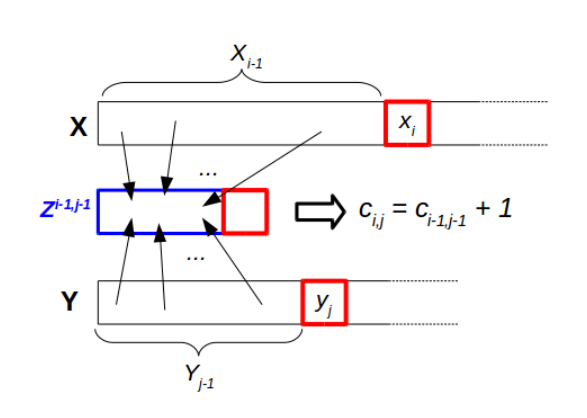
\includegraphics[width = 0.50\linewidth]{Images/5.png}
    \end{center}
    quindi $c_{i,j} = 1 + c_{i-1, j-1} \; \; \textrm{se } x_i = y_j$
    \item Se $x_i \neq y_j$ i due elementi considerati sono differenti, allora la lunghezza della più lunga sottosequenza comune è data dalla soluzione di uno dei sottoproblemi di dimensione minore.
    Siccome gli elementi finali dei due prefissi considerati sono differenti, non possono appartenere entrambi alla soluzione $Z_k$ e risulta necessario considerare i seguenti due casi, sulla base di come è fatto l'ultimo elemento $z_k$ della soluzione $Z_k$:
    \begin{itemize}
        \item Se $z_k \neq x_i$, allora si deve considerare la soluzione $c_{i-1,j}$, ossia la soluzione del sottoproblema di dimensione $(i-1,j)$ con input il prefisso $X_{i-1}$ e il prefisso $Y_j$
        \item Se $z_k \neq y_j$, allora si deve considerare la soluzione $c_{i,j-1}$, ossia la soluzione del sottoproblema di dimensione $(i,j-1)$ con input il prefisso $X_i$ e il prefisso $Y_{j-1}$
    \end{itemize}
    Siccome $z_k$ non è noto, non possiamo sapere a priori quale dei due casi si verifichi. Quindi consideriamo la soluzione di entrambi i sottoproblemi di dimensione $(i-1,j)$ e $(i, j-1)$ e scegliamo quella di valore massimo.
    Formalmente, possiamo scrivere:
    $$c_{i,j} = \max\{c_{i-1,j}, c_{i,j-1}\} \; \; se x_i \neq y_j$$
\end{itemize}
Il passo ricorsivo è quindi descrivibile come:
$$c_{i,j} = \begin{cases}
    1 + c_{i-1,j-1} \; \; \textrm{se } x_i = y_j \\
    \max\{c_{i-1,j}, c_{i, j-1}\} \; \; \textrm{se } x_i \neq y_j
\end{cases}$$
Una volta calcolati i valori di tutte le soluzioni ($c_{0,0}, c_{0,1}, \dots, c_{m,n}$), si hanno a disposizione tutte le lunghezza delle
sottosequenze comuni massimali fra qualsiasi prefisso di $X$ e qualsiasi prefisso di $Y$. La \textbf{soluzione del problema ridotto} è quindi
$$c_{m,n}$$
\begin{center}
    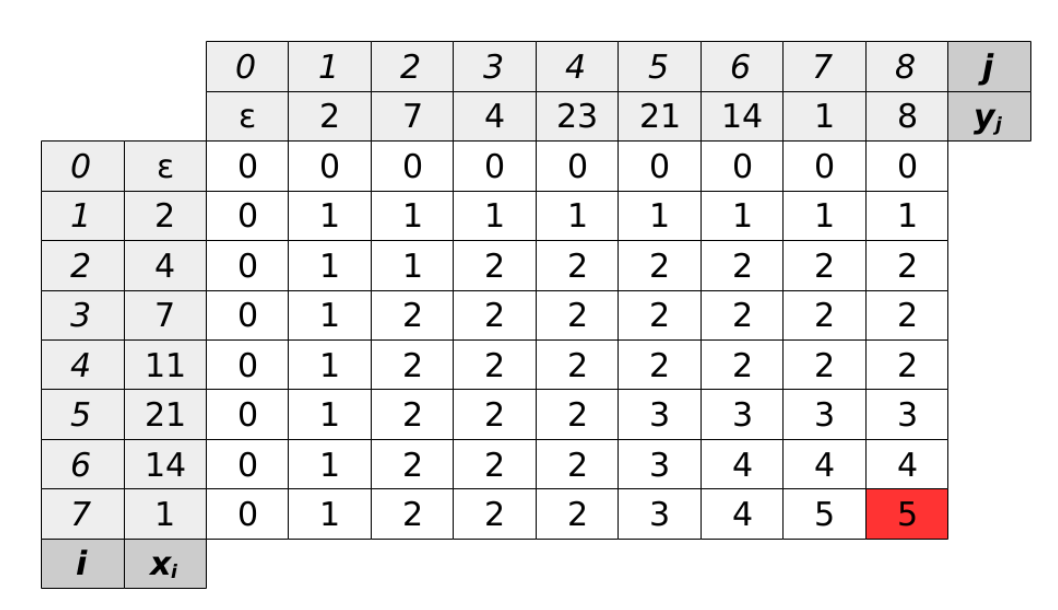
\includegraphics[width = 0.70\linewidth]{Images/6.png}
\end{center}
Scriviamo quindi l'algoritmo bottom-up per calcolare la lunghezza di una LCS fra $X$ e $Y$
\begin{algorithm}[H]
    \DontPrintSemicolon
    \caption{Algoritmo iterativo che calcola la lunghezza di una LCS di $X$ e $Y$}
    \SetKwFunction{FLCSLen}{LCS-LEN}
    \Proc{\FLCSLen{X,Y}} {
        m := LENGTH(X) \;
        n := LENGTH(Y) \;
        \For{$j \gets 0$ to $n$} {
            c[0,j] := 0
        }
        \For{$i \gets 0$ to $m$} {
            c[0,j] := 0
        }
        \For{$i \gets 1$ to $m$} {
            \For{$j \gets 1$ to $n$} {
                \eIf{$x_i = y_j$} {
                    c[i,j] := c[i-1, j-1] + 1 \;
                    b[i,j] := "$\nwarrow$" \;
                } {
                    \eIf{$c[i-1, j] \geq c[i, j-1]$} {
                        c[i,j] := c[i-1,j] \;
                        b[i,j] := "$\uparrow$" \;
                    } {
                        c[i,j] := c[i, j-1] \;
                        b[i,j] := "$\leftarrow$"
                    }
                }
            }
        }
        \Return c e b
    }
\end{algorithm} \noindent
Questo algoritmo ha lo stesso costo computazionale dell'algoritmo 4, cioè $T(n) = \Theta(m \cdot n)$.
Si noti che si utilizza una matrice ausiliaria $b$ di dimensioni $m \times n$ per memorizzare \textbf{l'informazione utile a ricostruire una LCS di $X$ e $Y$}; in 
particolare, andremo a salvare \textbf{quale sottoproblema è stato usato} tramite una freccia:
\begin{itemize}
    \item $\uparrow$ indica che è stato usato il sottoproblema $(i-1, j)$
    \item $\leftarrow$ indica che è stato usato il sottoproblema $(i, j-1)$
    \item $\nwarrow$ indica che è stato usato il sottoproblema $(i-1, j-1)$
\end{itemize}
Tramite la matrice $b$, abbiamo tutte le informazioni necessarie per definire un algoritmo ricorsivo che
\textbf{ricostruisca una LCS di $X$ e $Y$}: \newline
\begin{algorithm}[H]
    \caption{Algoritmo ricorsivo che stampa una LCS di $X$ e $Y$}
    \DontPrintSemicolon
    \SetKwFunction{FPrintLCS}{PRINT-LCS}
    \Proc{\FPrintLCS{b, X, i, j}} {
        \If{$i \neq 0 \land j \neq 0$} {
            \eIf{$b[i,j] = "\nwarrow"$} {
                PRINT-LCS(X, b, i-1, j-1) \;
                Print($x_i$) \;
            } {
                \eIf{$b[i,j] = "\uparrow"$} {
                    PRINT-LCS(X, b, i-1, j)\;
                } {
                    PRINT-LCS(X, b, i, j-1)\;
                }
            }
        }
    }
\end{algorithm}\noindent
La procedura impiega un tempo $T(n) = \Theta(m + n)$ perché a ogni chiamata ricorsiva essa decrementa almeno uno dei valori $i$ e $j$.
\subsection{WIS - Weighted Interval Scheduling}
Sia $X = \{1,\dots,n\}$ un insieme di $n$ attività, con $n \in \mathbb{N}$. Ad ogni attività
$i \in X$ sono associate le seguente informazioni $([s_i, e_i), v_i)$ dove:
\begin{itemize}
    \item $s_i$ indica il tempo di inizio dell'attività
    \item $e_i$ con $e_i \geq s_i$ indica il tempo di fine dell'attività (si noti che $e_i$ non appartiene all'intervallo che specifica la durata dell'attività)
    \item $v_i$ indica il valore dell'attività
\end{itemize}
Due attività $i,j \in X$ sono dette \textbf{compatibili} se non si sovrappongono:
$$[s_i, e_i) \cap [s_j, e_j) = \emptyset$$
Un insieme $X$ di attività \textbf{contiene attività mutualmente compatibili} se e solo se per tutte le coppie $(i,j)$ con $i \neq j$, l'attività $i$ è compatibile con l'attività $j$:
$$\forall i,j \in X \; \textrm{con } i \neq j, \textrm{se } [s_i, e_i) \cap [s_j, e_j) = \emptyset$$
Definiamo ora la seguente funzione:
$$COMP: \mathcal{P}(\{1,\dots,n\}) \rightarrow \{True, False\}$$
che associa ad ogni sottoinsieme di attività $A \subseteq \{1,\dots,n\}$, \textbf{True} se $X$ contiene
attività mutualmente compatibili, \textbf{False} altrimenti. Formalmente: $\forall A \subseteq \{1,\dots,n\}$:
$$COMP(A) = \begin{cases}
    True \; \; \; \textrm{se } \forall i,j \in A \; \textrm{con } i \neq j, [s_i, e_i) \cap [s_j, e_j) = \emptyset \\
    False \; \; \textrm{Altrimenti}
\end{cases}$$
Infine, definiamo la funzione
$$V: \mathcal{P}(\{1,\dots,n\}) \rightarrow \mathbb{R}^+$$
che associa ad ogni sottoinsieme di attività $A \subseteq \{1,\dots,n\}$ il suo valore complessivo.
Formalmente, $\forall A \subseteq \{1,\dots,n\}$:
$$V(A) = \begin{cases}
    \sum_{i\in A} v_i \; \; \textrm{se } A \neq \emptyset \\
    0 \; \; \; \; \; \; \; \; \; \; \; \; \textrm{Altrimenti}
\end{cases}$$
Definiamo quindi il problema: \newline
\textbf{\underline{PROBLEMA}}: Dato un insieme $\{1,\dots,n\}$ di attività, trovare un sottoinsieme di attività mutualmente compatibili di valore massimo \newline
\textbf{\underline{ISTANZA}}: $\{1,\dots,n\}$ con $([s_i, e:i), v_i) \; \forall i \in \{1,\dots,n\}$ \newline
\textbf{\underline{SOLUZIONE}}: $S \subseteq \{1,\dots,n\}$ tale che:
$$COMP(S) = TRUE \land V(S) = \max_{COMP(A) = TRUE}\{V(A)| A \subseteq X\}$$
Possiamo direttamente risolvere questo problema \textbf{senza definire un problema ridotto}.
Il problema contiene \textbf{diversi sottoproblemi}, ognuno dei quali non ha come input l'insieme $X$ con $([s_i, e_i) _i), \forall i \in X$ ma un suo sottoinsieme.
Formuliamo quindi il problema in modo \textbf{ricorsivo}:
\begin{enumerate}
    \item Dato $X_n = \{1,\dots,n\}$ si vuole trovare una soluzione $S_n \subseteq X_n$ tale che:
    $$COMP(S_n) = True \land V(S_n) = \max_{COMP(A) = True}\{V(A)|A \subseteq X_n\}$$
    \item Dato $X_{n-1} = \{1,\dots,n-1\}$ si vuole trovare una soluzione $S_{n-1} \subseteq X_{n-1}$ tale che:
    $$COMP(S_{n-1}) = True \land V(S_{n-1}) = \max_{COMP(A) = True}\{V(A)|A \subseteq X_{n-1}\}$$
    \item $\dots$
    \item Dato $X_2 = \{1,2\}$ si vuole trovare una soluzione $S_2 \subseteq X_2$ tale che:
    $$COMP(S_2) = True \land V(S_2) = \max_{COMP(A) = True}\{V(A)|A \subseteq X_2\}$$
    \item Dato $X_1 = \{1\}$ si vuole trovare una soluzione $S_1 \subseteq X_1$ tale che:
    $$COMP(S_1) = True \land V(S_1) = \max_{COMP(A) = True}\{V(A)|A \subseteq X_1\}$$
    \item Dato $X_0 = \emptyset$ si vuole trovare una soluzione $S_0 \subseteq X_0$ tale che:
    $$COMP(S_0) = True \land V(S_0) = \max_{COMP(A) = True}\{V(A)|A \subseteq X_0\}$$
\end{enumerate}
Quindi, \textbf{il generico sottoproblema del problema originale è individuato} da $i \in \{1,\dots, n\}$; il \textbf{sottoproblema di dimensione $i$ è definito come segue}: \newline
\textbf{\underline{SOTTOPROBLEMA GENERICO}}: Dato un insieme $\{1,\dots, n\}$ di attività, trovare un suo sottoinsieme di attività mutualmente compatibili di valore massimo \newline
Ossia: \newline
\textbf{\underline{ISTANZA DEL SOTTOPROBLEMA}}: $X_i = \{1,\dots, i\}$ con $([s_i, e_i), v_j) \; \forall i \in X_i$ \newline
\textbf{\underline{SOLUZIONE DEL SOTTOPROBLEMA}}: $S_i \subseteq X_i$ tale che:
$$COMP(S_i) = True \land V(S_i) = \max_{COMP(A) = True}\{V(A)|A \subseteq X_i\}$$
Dato che $0 \leq i \leq n$ si ottengono $(n+1)$ sottoproblemi, ad ognuno dei quali è associata una \textbf{coppia di variabili}:
considerato il sottoproblema di dimensione $i$, la coppia di variabili ad esso associata è $(OPT_i, S_i)$ ed è cosi definita:
\begin{center}
    $S_i$, un sottoinsieme di $X_i$ che contiene attività compatibili di peso massimo
    $OPT_i = V(S_i)$, ossia il valore di un sottoinsieme di $X_i$ che contiene attività mutualmente compatibili di peso massimo \\
\end{center}
Per determinare la soluzione di un qualsiasi sottoproblema di dimensione $i$, oltre all'input del problema, si utilizzeranno le soluzione dei sottoproblemi di dimensione minore e le loro variabili associate $S_j$ e $OPT_j$.
Si noti, però, che ognuna di queste variabili è da considerare come una \textbf{black-box}: si può utilizzare ma non è possibile conoscerne il contenuto.
Scriviamo quindi l'equazione di ricorrenza del problema: \newline
\textbf{\underline{CASO BASE}}: $i = 0$ \newline
Il caso vase si ha per un qualunque sottoproblema di dimensione $i = 0$, ossia quando non ci sono attività da considerare. In questo caso è facile ottenere la soluzione del sottoproblema:
$$OPT_i = 0$$
$$S_i = \emptyset$$
Dunque il caso base è descrivibile come:
$$OPT_i = 0 \; \textrm{e } S_i = \emptyset \; \; \textrm{se } i = 0$$
\textbf{\underline{PASSO RICORSIVO}}: $i > 0$
Per definire il passo ricorsivo, assumiamo che le attività in $X_n = \{1,\dots,n\}$ siano ordinate rispetto ai \textbf{tempi di fine}, cioè che valga che \newline $e_1 \leq e_2 \leq \dots \leq e_i \leq \dots \leq e_n$. Inoltre, dato
$i \in X_n$, definiamo:
$$\psi(i) = \max\{j|j < i \; \textrm{e } j \; \textrm{è compatibile con } i\}$$
Assumiamo infine che $\max \emptyset = 0$. \newline
Ora possiamo definire il passo ricorsivo. Esso si ha per un qualunque sottoproblema di dimensione $i$ con $i > 0$, ossia quando si va a considerare un insieme che contiene almeno un'attività.
I dati disponibili per calcolare la soluzione di un sottoproblema sono: l'input $X_i = \{1,\dots,i\}$ (in particolare l'attività $i$) e tutte le soluzioni dei sottoproblemi di dimensione minore.
Per risolvere un sottoproblema è necessario domandarsi: "Com'è fatto $S_i$ rispetto a $S_{i-1}, S_{i-2}, \dots, S_1, S_0$?" Per rispondere a questa domanda, bisogna considerare due casi:
\begin{itemize}
    \item Se $i \notin S_i$, cioè se l'attività $i$ non appartiene alla soluzione, allora è sufficiente considerare l'insieme di attività $X_{i-1} = \{1,\dots, i-1\}$ e si può dunque considerare la soluzione del sottoproblema di dimensione subito minore, ossia:
    $$OPT_i = OPT_{i-1} \; e \; S_i = S_{i-1}$$
    \item Se $i \in S_i$, cioè se l'attività $i$ appartiene alla soluzione, allora è necessario andare a determinare la soluzione del sottoproblema di dimensione minore ad $i$ di peso massimo e il cui insieme di attività risulta essere compatible con l'attività $i$.
    È dunque possibile considerare la soluzione del sottoproblema di dimensione $\psi(i)$ e aggiungere a questa attività $i$. Si ottiene dunque:
    $$OPT_i = OPT_{\psi(i)} + v_i \; e \; S_i = S_{\psi(i)} \cup \{i\}$$
\end{itemize}
Siccome non possiamo sapere a priori se l'attività $i$ appartenga o meno alla soluzione, consideriamo \textbf{entrambe le soluzioni e scegliamo quella di valore massimo}.
Formalmente possiamo scrivere:
$$OPT_i = \max\{OPT_{i-1}, OPT_{\psi(i)} + v_i\}$$
e
$$S_i = \begin{cases}
    S_{i-1} \; \; \, \; \; \; \; \; \; \; \; \; \textrm{se } OPT_{i-1} \geq OPT_{\psi(i)} + v_i \\
    S_{\psi(i)} \cup \{i\} \; \; \textrm{Altrimenti}
\end{cases}$$
Si noti come l'insieme $S_i$ venga definito a partire dalle variabili $S_j$ ma sulla base dei valori delle variabili $OPT_j$ relative ai sottoproblemi di dimensione minore (ossia con $j < i$).
Una volta calcolati i valori $OPT_0, OPT_1, \dots, OPT_n$, è possibile determinare la \textbf{soluzione del problema} andando a considerare la coppia:
$$(OPT_n, S_n)$$
\begin{center}
    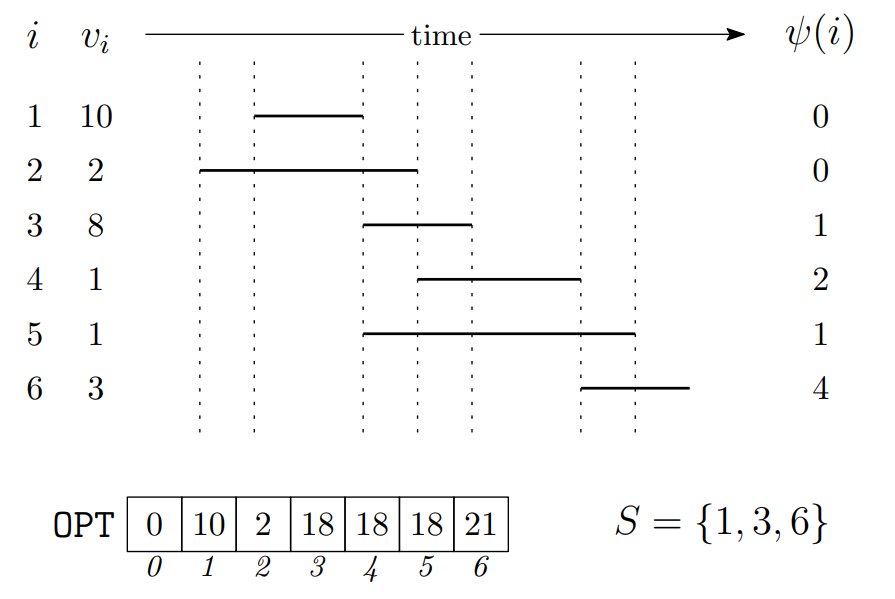
\includegraphics[width = 0.60\linewidth]{Images/7.png}
\end{center}
Enunciamo quindi il teorema della \textbf{proprietà della sottostruttura ottima}:
\begin{Teorema}[PSO di WIS]
    Sia $i \geq 1$. Siano $S_0, S_1, \dots, S_{i-1}$ soluzioni dei sottoproblemi di dimensione $0, 1,\dots,i-1$ di WIS.
    Allora vale che:
    \begin{equation*}
        S_i = \begin{cases}
        S_{\psi(i)} \cup \{i\} & \textrm{se } i \in S_i \\
        S_{i-1} & \textrm{se } i \notin S_i
    \end{cases}
    \end{equation*}
\end{Teorema}
\begin{Dimostrazione}
    Distinguiamo i due casi:
    \begin{itemize}
        \item Supponiamo che $i \notin S_i$; devo allora dimostrare che $S_i = S_{i-1}$.
        Supponiamo per assurdo che $S_{i-1}$ non sia soluzione del problema $i$, cioè $S_i \neq S_{i-1}$.
        Allora esiste $S' \neq S_{i-1}$ che è soluzione del problema $i$; allora $V(S') > V(S_{i-1})$.
        Inoltre $i \neq S' rightarrow S' \subseteq\{1,\dots, i-1\}$, ma allora $S_{i-1}$ non potrebbe essere la soluzione
        del sottoproblema $i-1$, \textbf{assurdo}!.
        \item Supponiamo che $i \in S_i$; devo dimostrare che $S_i = S_{\psi(i)} \cup \{i\}$
        Supponiamo per assurdo che $S_i \neq S_{\psi(i)} \cup \{i\}$ e che quindi $S_{\psi(i)} \cup \{i\}$ non è soluzione del problema $i$.
        Allora esiste $S' \neq S_{\psi(i)} \cup \{i\}$ che è soluzione del problema $i$; allora $V(S') > V(S_{\psi(i)} \cup \{i\})$.
        Inoltre $i \in S'$, quindi $S' = S'' \cup \{i\}$ con $S''$ formato da attività mutualmente compatibili.
        Inoltre $S'' \subseteq \{1,\dots, \psi(i)\}$, quindi:
        $$V(S') = V(S'') + v_i > V(S_{\psi(i)}) + v_i = V(S_{\psi(i)} \cup \{i\})$$
        cioè
        $$V(S'') > V(S_{\psi(i)})$$
        ma quindi $S_{\psi(i)}$ non può essere soluzione del sottoproblema $S_{\psi(i)}$, \textbf{assurdo}!
    \end{itemize}
\end{Dimostrazione}
Utilizzando le equazioni di ricorrenza presentate precedentemente, possiamo definire in maniera immediata un algoritmo ricorsivo che
ritorni \textbf{la soluzione di ogni sottoproblema}: \newline
\begin{algorithm}[H]
    \caption{Algoritmo ricorsivo che ritorna la soluzione del problema WIS}
    \SetKwFunction{FWISRic}{WIS-Ric}
    \Proc{\FWISRic{i}} {
        \eIf{$i = 0$} {
            \Return (0, $\emptyset$)
        } {
            $(V_1, S_1) \gets \textrm{WIS-Ric}(i-1)$ \;
            $(V_2, S_2) \gets \textrm{WIS-Ric}(\psi(i))$ \;
            $V_2 \gets V_2 + v_i$ \;
            \eIf{$V_1 \geq V_2$} {
                \Return $(V_1, S_1)$
            } {
                \Return $(V_2, S_2 \cup \{i\})$
            }
        }
    }
\end{algorithm} \noindent
Questo algoritmo \textbf{ha complessità esponenziale}, dato che ogni sottoproblema viene risolto più volte. 
È Anche facile scrivere un algoritmo ricorsivo che calcoli il valore di $OPT_i$: \newline
\begin{algorithm}[H]
    \caption{Algoritmo ricorsivo che calcola il valore di $OPT_i$}
    \SetKwFunction{FOPTRic}{OPT-Ric}
    \Proc{\FOPTRic{i}} {
        \eIf{$i = 0$} {
            \Return 0
        } {
            \Return $\max \{\textrm{OPT-Ric}(\psi(i)) + v_i, \textrm{OPT-Ric}(i-1)\}$
        }
    }
\end{algorithm} \noindent
Possiamo utilizzare una tecnica \textbf{bottom-up} per risolvere il problema WIS: questa tecnica
infatti permette di calcolare la soluzione di ogni sottoproblema solo una volta. In questo modo si ottiene un algoritmo con \textbf{complessità spaziale maggiore}, in quanto devo memorizzare le varie soluzioni, ma con \textbf{complessità di tempo minore rispetto all'algoritmo ricorsivo}.
L'algoritmo bottom-up per il calcolo della soluzione del problema WIS è il seguente: \newline
Prima di tutto definisco un algoritmo iterativo per calcolare i valori di $OPT$ legati alle soluzioni; per farlo
mi avvalgo di un array $M$ di dimensione $n$: \newline
\begin{algorithm}[H]
    \caption{Algoritmo iterativo per il calcolo di $OPT$}
    \SetKwFunction{FOPTIt}{OPT-IT}
    \Proc{\FOPTIt{n}} {
        $M[0] := 0$ \;
        \For{$i \gets 1$ to $nell$} {
            $M[i] := \max\{M[\psi(i)] + v_i, M[i-1]\}$
        }
    }
\end{algorithm} \noindent
dopodiché definisco l'algoritmo bottom-up per il calcolo della soluzione al problema WIS: per farlo
mi avvalgo di un array $S$ di dimensione $n$ che contiene le soluzioni dei sottoproblemi (cioè gli insiemi di attività mutualmente compatibili) \newline
\begin{algorithm}[H]
    \caption{Algoritmo iterativo per il calcolo della soluzione del problema WIS}
    \SetKwFunction{FWISIt}{WIS-IT}
    \Proc{\FWISIt{n}} {
        $S := \emptyset$ \;
        \For{$i \gets 1$ to $n$} {
            $V_1 := M[i-1]$ \;
            $V_2 := M[\psi(i)] + v_i$ \;
            \eIf{$V_1 \geq V_2$} {
                $S[i] := S[i-1]$
            } {
                $S[i] := S[\psi(i)] \cup \{i\}$
            }
        }
        \Return $(M[n], S[n])$
    }
\end{algorithm} \noindent
\begin{algorithm}[H]
    \caption{Algoritmo di ricostruzione della soluzione di WIS}
    \DontPrintSemicolon
    \SetKwFunction{FPrintWIS}{PRINT-WIS}
    \Proc{\FPrintWIS{i, M}} {
        \If{$i \neq 0$} {
            \eIf{$M[\psi(i)] + v_i \geq M[i-1]$} {
                PRINT-WIS($\psi(i)$, $M$) \;
                Print($i$)
            } {
                PRINT-WIS($i-1$, $M$)
            }
        }
    }
\end{algorithm} \noindent
La complessità computazionale dell'algoritmo 10 è:
$$T(n) = \mathcal{O}(n)$$
tuttavia, esso occupa uno spazio in memoria pari a $\mathcal{O}(n + n^2)$ poiché necessita
di un vettore per contenere i vari $OPT_i$ e un vettore per contenere i vari insieme $S_i$, ognuno dei quali può contenere
al massimo $n$ elementi.
\subsection{LIS - Longest Increasing Subsequence}
Il problema LIS è definito come segue: \newline
\textbf{\underline{PROBLEMA}}: Data una sequenza $X$ di $n$ numeri interi, si determini \textbf{\underline{UNA}} tra le più lunghe sottosequenze strettamente crescenti di $X$. \newline
\textbf{\underline{ISTANZA}}: $X_n = <x_1, \dots, x_n>$ \newline
\textbf{\underline{SOLUZIONE}}: $Z$ una più lunga sottosequenza strettamente crescete di $X_n$ \newline
In particolare, come nel caso di LCS, andremo a risolvere un \textbf{problema ridotto}: \newline
\textbf{\underline{PROBLEMA RIDOTTO}}: Data una sequenza $X$ di $n$ numeri interi, si determini \textbf{la lunghezza} di una tra le più lunghe sottosequenze strettamente crescenti di $X$ \newline
Il problema ridotto contiene \textbf{diversi sottoproblemi} ognuno dei quali non ha come input la sequenza $X$ ma un suo prefisso.
Il \textbf{generico sottoproblema} di dimensione $i$ è definito come segue: \newline
\textbf{\underline{SOTTOPROBLEMA GENERICO}}: Data una sequenza $X$ di $n$ numeri interi, si determini la lunghezza di una tra le più lunghe sottosequenze strettamente crescenti di $X_i$. \newline
Dato che $1 \leq i \leq n$, si ottengono $n$ sottoproblemi (non si considera in questo caso il valore $i = 0$). Ad ogni sottoproblema del problema ridotto \textbf{è associata una variabile}: considerato il 
sottoproblema di dimensione $i$, la variabile ad esso associata è $c_i$, ed è così definita:
\begin{center}
    $c_i =$ lunghezza di una tra le più lunghe sottosequenze strettamente crescenti di $X_i$
\end{center}
Per determinare la soluzione di un qualsiasi sottoproblema di dimensione $i$, oltre all'input del problema, si utilizzeranno le soluzioni dei sottoproblemi di dimensione minore.
Proviamo ad impostare la risoluzione del problema come abbiamo fatto con LCS: siano allora:
\begin{center}
    $X_n = <x_1, \dots, x_n>$ \\
    $X_{n-1} = <x_1, \dots, x_{n-1}>$ \\
    $\dots$ \\
    $X_1 = <x_1>$ \\
    $X_0 = \varepsilon$
\end{center}
La soluzione allora potrebbe avere la seguente struttura:
$$S_n =S_{n-k}|x_n \; \; \textrm{con } 0 < k < n$$
per sapere se questa assunzione sia vera o meno, mi basterebbe sapere l'ultimo elemento di $S_{n-k}$; tuttavia
\textbf{NON POSSIAMO SAPERE IL VALORE DI $s_{n-k}$} poiché le soluzioni ai sottoproblemi sono delle \textbf{black-box} e quindi
\textbf{NON NE CONOSCIAMO IL VALORE!}. Per risolvere il problema dobbiamo quindi introdurre un \textbf{PROBLEMA VINCOLATO}: \newline
\textbf{\underline{PROBLEMA VINCOLATO}}: Data una sequenza $X$ di $n$ numeri interi, si determini la lunghezza di una tra le più lunghe sottosequenze strettamente crescenti
di $X$, la quale termina con $x_n$. \newline
In altre parole, si richiede che la sottosequenza crescente più lunga termini con l'ultimo elemento della sequenza di input.
Come per il problema ridotto, \textbf{anche il problema vincolato contiene $n$ diversi sottoproblemi}, ognuno associato ad una differente variabile.
Il sottoproblema generico del problema vincolato di dimensione $i$ è definito come segue: \newline
\textbf{\underline{SOTTPROB. GEN. PROBLEMA VINCOLATO}}: Data una sequenza $X$ di $n$ numeri interi, si determini la lunghezza di una tra le più lunghe sottosequenze strettamente crescenti di $X_i$, la quale termina con $x_i$ \newline
ogni sottoproblema generico è associato ad una variabile $c_i$ così definita:
\begin{center}
    $c_i = $ lunghezza di una tra le più lunghe sottosequenze crescenti di $X_i$, la quale termina con $x_i$
\end{center}
Si noti quindi che per un qualunque sottoproblema di dimensione $s$, solo imponendo che la soluzione $c_s$ si riferisca ad una sottosequenza strettamente crescente
di $X_s$ la quale termina con $x_s$ è possibile stabilire se un altro elemento $x_u$ con $u > s$ possa essere accodato a tale sottosequenza (andando a verificare che $x_s < x_u$). \newline
Prima di procedere con le equazioni di ricorrenza, può essere utile enunciare e dimostrare già adesso il teorema della proprietà della sottostruttura ottima \textbf{per il problema vincolato}:
\begin{Teorema}[PSO LIS Vincolato]
    Sia $X$ una sequenza di $n$ numeri interi e sia $X_i$ un suo prefisso di lunghezza $i$ con $1 \leq i \leq n$. Sia $Z^i$ una tra le più lunghe sottosequenze strettamente crescenti di $X_i$ la quale termina
    con $x_i$. Allora vale che $Z^i = Z^*|x_i$, con $Z^* \in \mathcal{W}_i$ e $|Z^*| = \max_{W \in \mathcal{W}_i}\{|W|\}$, dove $\mathcal{W}_i$ è l'insieme di tutte le sottosequenze crescenti (\textbf{non necessariamente più lunghe}) di $X_j$ le quali finiscono con $x_j$ e a cui è possibile
    concatenare $x_i$, ovvero:
    $$\mathcal{W}_i = \smashoperator[r]{\bigcup_{\substack{1 \leq j \leq i \\ x_j < x_i}}}\{W \; \textrm{sottosequenza di } X_j \; \textrm{la quale termina con } x_j\}$$
\end{Teorema}
Si noti che $Z^*$ \textbf{sarà anche soluzione di un qualche sottoproblema di dimensione minore a $i$} (una più lunga tra le soluzioni di alcuni sottoproblemi più piccoli, in particolare quei sottoproblemi $j < i$ tali che $x_j < x_i$).
\begin{Dimostrazione}
    Per assurdo, si supponga che $Z^*|x_i$ non sia la soluzione del problema $i$-esimo. Allora, relativamente alla soluzione $Z^i$ del problema valgono le seguente affermazioni:
    \begin{enumerate}
        \item $Z'$ tale che $Z^i = Z'|x_i$
        \item $|Z'| > |Z^*|$ (dato che $Z^i$ non si ottiene a partire da $Z^*$ ma da $Z'$, necessariamente $Z'$ sarà più lunga di $Z^*$)
    \end{enumerate}
    Dove $Z'$ è una qualche sottosequenza crescente di un prefisso più piccolo di $X_i$. Sia ora $z'$ l'ultimo elemento di $Z'$. Vale quindi che $z' < x_i$ poiché è stato
    possibile concatenare $x_i$ a $Z'$. Inoltre, sia $h < i$ \textbf{il più grande indice tale che $x_h = z'$}. Di conseguenze, per come è stato definito $\mathcal{W}_i$, si ottiene
    che $Z' \in \mathcal{W}_i$. Infatti $Z'$ è una \textbf{sottosequenza strettamente crescente } di $X_h$, la quale termina con $x_h < x_i$.
    Ciò pero porta ad una contraddizione: infatti dal punto 2 vale che $|Z'| > |Z^*|$, ma ciò non può valere con l'ipotesi che $|Z*| = \max_{W \in \mathcal{W}_i}\{|W|\}$, quindi \textbf{assurdo}!
\end{Dimostrazione}
Scriviamo ora le equazioni di ricorrenza: \newline
\textbf{\underline{CASO BASE}}: $i = 1$ \newline
Il caso base si ha quando $i = 1$, ossia quando il prefisso considerato è una sequenza composta da un singolo elemento.
È facile ottenere il valore della variabile $c_1$: la lunghezza di una tra le più lunghe sottosequenze crescenti di una sequenza composta da un singolo elemento la quale termina con quell'elemento è $1$. Il caso base è quindi scrivibile come:
$$c_i = 1 \; \textrm{se } i = 1$$
\textbf{\underline{PASSO RICORSIVO}}: $i > 1$ \newline
Il passo ricorsivo si ha per un qualunque sottoproblema di dimensione $i$ con $i >1$, ossia quando si considera un prefisso della sequenza $X$ in input di almeno due elementi.
I dati disponibili per calcolare $c_i$ sono: l'input $X$ ed in particolare l'elemento $x_i$ e tutte le variabili $\{c_1,\dots,c_{i-1}\}$. Si ricorda che i valori $c_1,c_2,\dots,c_{i-1}$ rappresentano
\textbf{le lunghezza delle più lunghe sottosequenze strettamente crescenti di $X_1, X_2, \dots, X_{i-1}$} le quali terminano rispettivamente con $x_1, x_2, \dots, x_{i-1}$.
Tra queste ci saranno alcune sottosequenze alle quali possiamo accodare $x_i$ (in quanto maggiore dell'ultimo elemento) e altre alle quali l'elemento $x_i$ non può essere accodato (in quanto minore dell'ultimo elemento).
Se prendiamo la più lunga sottosequenza strettamente crescente alla quale possiamo attaccare $x_i$ e accodiamo ad essa $x_i$, otteniamo la più lunga sottosequenza strettamente crescete di $X_i$ che termina con $x_i$.
La lunghezza di tale sottosequenza sarà uguale alla lunghezza della sottosequenza crescente alla quale abbiamo accodato $x_i$ aumentata di 1. Il passo ricorsivo è quindi scrivibile come:
$$c_i = 1 + \max\{c_h|1 \leq i \land x_h < x_i \}$$
Poiché può accadere che l'insieme $\{c_h|1 \leq i \land x_h < x_i \}$ \textbf{sia vuoto} (il che corrisponde al fatto che l'elemento $x_i$ è minore di tutti gli elementi precedenti e, quindi, non può essere accodato a nessuna più lunga sottosequenza strettamente crescente relativa a sottoproblemi di dimensione minore),
assumiamo per definizione che $\max \emptyset = 0$, così che il corrispondente valore di $c_i$ risulti uguale a 1 in questo caso.
\begin{center}
    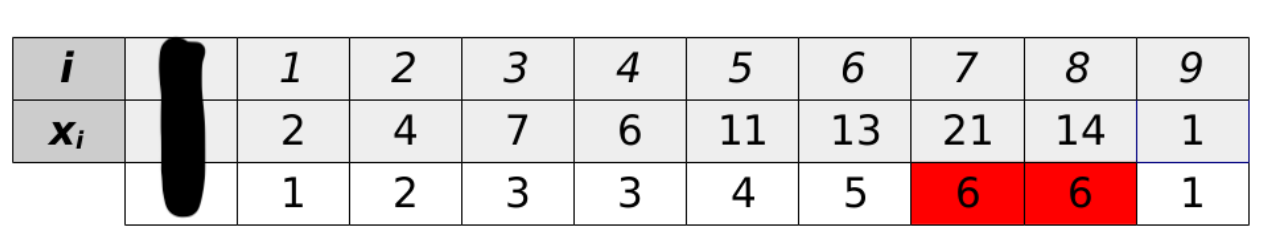
\includegraphics[width = 0.60\linewidth]{Images/8.png}
\end{center}
Una volta calcolati i valori $c_1, \dots, c_n$ si hanno a disposizione tutte le lunghezze di una tra le più lunghe sottosequenze crescenti dei vari prefissi di $X$ le quali terminano
con l'ultimo elemento del prefisso. La \textbf{soluzione del problema vincolato} è $c_n$, mentre \textbf{la soluzione del problema ridotto} è:
$$\max\{c_i|1 \leq i \leq n\}$$
Con le informazioni presentate fino ad ora, è immediato ricavare l'algoritmo ricorsivo per determinare la soluzione $c_i$ di ogni sottoproblema (si suppone di aver accesso alla sequenza $X$). In ogni caso, questo algoritmo
\textbf{presenterà una complessità esponenziale}, dato che ogni sottoproblema viene risolto più volte. \newline
\begin{algorithm}[H]
    \caption{Algoritmo ricorsivo per risolvere un sottoproblema $i$ di LIS}
    \DontPrintSemicolon
    \SetKwFunction{FLISRic}{LIS-Ric}
    \Proc{\FLISRic{i}} {
        \eIf{$i = 1$} {
            \Return 1
        } {
            $max := 0$ \;
            \For{$h \gets 1$ to $i-1$} {
                \If{$x_h < x_i$} {
                    $S := $ LIS-Ric(h) \;
                    \If{$S > max$} {
                        $max = S$
                    }
                }
            }
            \Return $1 + max$
        }
    }
\end{algorithm} \noindent
Possiamo quindi scrivere un algoritmo bottom-up per risolvere il problema. Utilizziamo
anche un array $b$ per salvare dati utili alla ricostruzione. \newline
\begin{algorithm}[H]
    \caption{Algoritmo iterativo che calcola una LIS di una sequenza $X$}
    \DontPrintSemicolon
    \SetKwFunction{FLISIt}{LIS-IT}
    \Proc{\FLISIt{X}} {
        $c[1] := 1$ \;
        $b[1] := 0$ \;
        $max := c[1]$ \;
        \For{$i \gets 2$ to $n$} {
            $tmp := 0$ \;
            $ind := 0$ \;
            \For{$h \gets 1$ to $i-1$} {
                \If{$(x_h < x_i) \land (c[h] > temp)$} {
                    $temp := c[h]$ \;
                    $ind := h$
                }
                $c[i] :=  1 + temp$ \;
                $b[i] := ind$ \;
                \If{$c[i] > max$} {
                    $max := c[i]$ \;
                    $indMax := i$
                }
            }
        }
        \Return $max$
    }
\end{algorithm}\noindent
L'algoritmo ha complessità computazionale
$$T(n) = \mathcal{O}(n^2)$$
e occupa spazio in memoria pari a $\Theta(n)$ (ossia un vettore che contiene i vari $c_i$; ovviamente non stiamo contando il vettore introdotto per la ricostruzione).
L'algoritmo ricorsivo per la ricostruire la LIS è il seguente: \newline
\begin{algorithm}[H] 
    \caption{Algoritmo di ricostruzione di una LIS di $X$}
    \DontPrintSemicolon
    \SetKwFunction{FPRINTLis}{PRINT-LIS}
    \Proc{\FPRINTLis{i, b, X}} {
        \eIf{$b[i] \neq 0$} {
            PRINT-LIS($b[i]$, $b$, $X$) \;
            Print($x_i$) \;
        } {
            Print($x_i$)
        }
    }
\end{algorithm} \noindent
Notare che per ottenere una LIS di $X$ è necessario sapere \textbf{in che indice dell'array $c$ è presente la massima lunghezza calcolata}; cioè bisogna
sapere quale numero, se messo in coda, porta a formare una più lunga sottosequenza strettamente crescente di $X$ (ovviamente ce ne potrebbero essere più di uno, ma noi
ne basta uno). Nell'algoritmo bottom-up lo abbiamo salvato nella variabile $indMax$.
\subsection{LICS - Longest Increasing Common Subsequence}
Il problema LICS è definito come segue: \newline
\textbf{\underline{PROBLEMA}}: Date due sequenze $X$ e $Y$, rispettivamente di $m$ ed $n$ numeri interi, si determini \textbf{\underline{UNA}} tra le più lunghe sottosequenze crescenti comuni a $X$ e $Y$. \newline
\textbf{\underline{ISTANZA}}: $X_m = <x_1, \dots, x_m>$ e $Y_n = <y_1, \dots, y_n>$ \newline
\textbf{\underline{SOLUZIONE}}: Una più lunga sottosequenza crescente di $X_m$ e $Y_n$. \newline
Quello che si andrà a risolvere sarà comunque un \textbf{problema ridotto}, il quale è definito come segue: \newline
\textbf{\underline{PROBLEMA RIDOTTO}}: Date due sequenze $X$ e $Y$, rispettivamente di $m$ ed $n$ numeri interi, si determini
la \underline{lunghezza} di una tra le più lunghe sottosequenze crescenti comuni a $X$ e $Y$. \newline
Il problema ridotto contiene diversi sottoproblemi, ognuno dei quali non ha come input la coppia $(X, Y)$ ma una \textbf{coppia di prefissi} di tali sequenze.
Il sottoproblema generico è quindi individuato dalla coppia $(i,j)$ ed è definito come segue: \newline
\textbf{\underline{SOTTOPROBLEMA GENERICO}}: Date due sequenze $X$ e $Y$, rispettivamente di $m$ ed $n$ numeri interi, si determini la lunghezza di una tra le più lunghe sottosequenze crescenti comuni
al prefisso $X_i$ e al prefisso $Y_j$. \newline
Non consideriamo coppie $(i,j)$ con $i = 0 \vee j = 0$. Dato che $1 \leq i \leq m$ e $1 \leq j \leq n$, si ottengono $m \cdot n$ sottoproblemi.
Ad ogni sottoproblema \textbf{è associata una variabile}: considerato il sottoproblema di dimensione $(i,j)$, la variabile ad esso associata è $c_{i,j}$ così definita:
\begin{center}
    $c_{i,j} =$ lunghezza di una tra le più lunghe sottosequenze crescenti comuni a $X_i$ e $Y_j$
\end{center}
per determinare la soluzione di un qualsiasi sottoproblema di dimensione $(i,j)$, oltre all'input del problema, si utilizzeranno anche le soluzioni dei sottoproblemi di dimensione minore.
Si noti, però, che ognuna delle variabili associate ai diversi sottoproblemi è da considerare come una \textbf{black-box}: si può utilizzare ma non è possibile conoscerne il contenuto. \newline
Proviamo ad approcciarci al problema come abbiamo fatto con LCS: se $x_i = y_j$, la struttura della soluzione potrebbe essere:
$$S^{(i,j)} = S|x_i$$
con $S$ una soluzione di un sottoproblema di dimensione minore. Tuttavia, \textbf{non sappiamo cosa è contenuto all'interno di $S$}, quindi \textbf{ci mancano delle informazioni necessarie per continuare}.
Infatti, date solamente le variabili $\{c_{1,1}, \dots, c_{i-1, j}, c_{i, j-1}\}$ e i prefissi $X_i$ e $Y_j$ (dei quali, in realtà, ci interessano solamente gli elementi $x_i$ e $y_j$), non c'è alcun modo per poter comprendere
se gli elementi $x_i$ e $y_j$, nel caso fossero uguali, possano essere accodati alle sottosequenze crescenti relative ai sottoproblemi di dimensioni minore a $(i,j)$: non sappiamo infatti con quale elemento termini ognuna di queste sottosequenze ma ne conosciamo
solamente la lunghezza (nel caso del problema ridotto). Si rende quindi necessaria l'introduzione di un \textbf{problema ausiliario} nel quale introdurre l'informazione mancante necessaria.
Il problema ausiliario è definito come segue: \newline
\textbf{\underline{PROBLEMA AUSILIARIO}}: Date due sequenze $X$ e $Y$, rispettivamente di $m$ ed $n$ numeri interi, si determina la lunghezza di una tra le più lunghe sottosequenze crescenti comuni a $X$ e $Y$ la quale termini
con $x_m$ e $y_n$ (se questi coincidono, 0 in caso contrario) \newline \newline
In altre parole, si richiede che la sottosequenza soluzione del problema termini con l'ultimo elemento delle sequenze $X$ e $Y$ nel caso siano lo stesso elemento (in caso contrario, \textbf{la soluzione non esiste}, il valore 0 per la lunghezza sta ad indicare tale fatto in questo contesto ed esso risulterà utile nel passo ricorsivo).
Come per il problema ridotto, anche il problema ausiliario contiene $m \cdot n$ diversi sottoproblemi, ognuno associato ad una differente variabile. Il sottoproblema generico del problema ausiliario di dimensione $(i,j)$ è definito come segue: \newline
\textbf{\underline{SOTTOPROB. GEN. PROB. AUSILIARIO}}: Date due sequenze $X$ ed $Y$, rispettivamente di $m$ ed $n$ numeri interi, si determini la lunghezza di una tra le più lunghe sottosequenze crescenti comuni a $X_i$ e $Y_j$ la quale termini con $x_i$ e $y_j$ (se questi coincidono). \newline
Anche in questo caso, ad ogni sottoproblema è associata una variabile $c_{i,j}$ così definita:
\begin{center}
    $c_{i,j} =$ lunghezza di una tra le più lunghe sottosequenze crescenti comuni a $X_i$ e $Y_j$ la quale termina con $x_i$ e $y_j$ (se questi coincidono, 0 altrimenti)
\end{center}
Si noti che per un qualunque sottoproblema di dimensione $(s,t)$, solo imponendo che la soluzione $c_{s,t}$ si riferisca ad una sottosequenza crescente comune a $X_s$ e $Y_t$ la quale termini con $x_s = y_t$ è possibile stabilire se un altro elemento $x_u = y_v$ con $u>s$ e $v>t$ possa essere
accodato a tale sottosequenza (andando a verificare che $x_s = y_t \leq x_u = y_v$). \newline
Prima di enunciare l'equazione di ricorrenza, può essere utile enunciare e dimostrare fin da subito il \textbf{teorema della proprietà della sottostruttura ottima per il problema ausiliario}:
\begin{Teorema}[PSO LICS Vincolata]
    Sia $X$ una sequenza di $m$ numeri interi e sia $X_i$ un suo prefisso di lunghezza $i$ con $1 \leq i \leq m$. Sia $Y$ una sequenza di $n$ numeri interi e sia $Y_j$ un suo prefisso di lunghezza
    $j$ con $1 \leq j \leq n$. Sia $Z^{(i,j)}$ una tra le più lunghe sottosequenze crescenti comuni di $X_i$ e $Y_j$ la quale termina con $x_i = y_j$. Allora vale che $Z^{(i,j)} = Z^*|x_i$ (analogamente, $Z^{(i,j)} = Z^*|y_j$) con $Z^* \in \mathcal{W}_{i,j}$ e $|Z^*| = \max_{W \in \mathcal{W}_{i,j}}\{|W|\}$ dove $\mathcal{W}_{i,j}$ è
    l'insieme di tutte le sottosequenze crescenti comuni (non necessariamente le più lunghe) di $X_h$ e $Y_k$ le quali terminano con $x_h = y_k$ e a cui è possibile concatenare $x_i$ (o analogamente $y_i$), ovvero:
    $$\mathcal{W}_{i,j} = \smashoperator[r]{\bigcup_{\substack{1 \leq h < i \\ 1 \leq k < j \\ x_h = y_k<x_i = y_j}}}\{W \textrm{sottosequenza crescente di } X_h \; e \; Y_k \; \textrm{che termina con } x_h = y_k\}$$
\end{Teorema}
Si noti che $Z^*$ sarà una soluzione di un qualche sottoproblema di dimensione minore a $(i,j)$ (una più lunga tra le soluzioni di alcuni sottoproblemi più piccoli, in particolare quei sottoproblemi $(h,k)$ con $h<i$ e $k<j$ tali che $x_h=y_k<x_i=y_j$).
\begin{Dimostrazione}
    Per assurdo supponiamo che $Z^*|x_i$ non sia la soluzione del problema $(i,j)-esimo$. Allora, relativamente alla soluzione $Z^{(i,j)}$ del problema valgono le seguenti affermazioni:
    \begin{enumerate}
        \item $Z^{(i,j)} = Z'|x_i$
        \item $|Z'| > |Z^*|$ (dato che $Z'$ non si ottiene a partire da $Z^*$ ma da $Z'$, necessariamente $Z'$ sarà più lunga di $Z^*$)
    \end{enumerate}
    Dove $Z'$ è una qualche sottosequenza comune crescente di un prefisso più piccolo di $X_i$ e $Y_j$. Sia ora $z'$ l'ultimo elemento di $Z'$, vale quindi che $z' < x_i =y_j$, poiché
    è stato possibile concatenare $x_i$ (o $y_j$) a $Z'$. Inoltre, siano $r < i$ e $s < j$ i \textbf{più grandi indici tali per cui $x_r = y_s = z'$}. Di conseguenza, per come è stato definito $\mathcal{W}_{i,j}$, si ottiene che $Z' \in \mathcal{W}_{i,j}$. Infatti
    $Z'$ è una sottosequenza comune crescente di $X_r$ e $Y_s$, la quale termina con $x_r < x_i$. Ciò però porta ad una contraddizione: infatti dal punto 2 vale che $|Z'| > |Z^*|$, ma ciò è in contraddizione con l'ipotesi che $|Z^*| = max_{W \in \mathcal{W}_{i,j}}\{|W|\}$,
    quindi è \textbf{assurdo}!.
\end{Dimostrazione}
Scriviamo ora \textbf{l'equazione di ricorrenza riferite al problema ausiliario}: \newline
\textbf{\underline{CASO BASE}}: Se $x_i \neq y_j$ \newline
Certamente fanno parte del caso bse tutte le coppie $(i,j)$ tali che $x_i \neq y_j$, ossia quando i due prefissi considerati $X_i$ e $Y_j$ terminano con due elementi diversi.
Questo caso, infatti, è semplice da risolvere: per definizione di $c_{i,j}$ gli elementi $x_i$ e $y_j$ devono coincidere, in caso contrario la soluzione è 0 (ossia non c'è nessuna sequenza soluzione).
Il numero di sottoproblemi che compone il problema ausiliario sono quindi $m \cdot n$. Il caso base si ha per quei \textbf{sottoproblemi di dimensione $(i,j)$ con $i > 0 \land j > 0$ tali che $x_i \neq y_j$} ed è scrivibile come segue:
$$c_{i,j} = 0$$
\begin{Nota}
    Quanti casi base invece esistono? \textbf{Dipende dalle sottosequenze}; infatti non posso saperlo a priori; l'unica informazione che ho al riguardo è che è un \textbf{numero in funzione dell'input}.
\end{Nota} \noindent
\textbf{\underline{PASSO RICORSIVO}}: $(i,j)$ con $i >0$ e $j>0$ tali che $x_i = y_j$ \newline
IL passo ricorsivo si ha per un qualunque sottoproblema $(i,j)$ tale che $x_i = y_j$, ossia quando i due prefissi $X_i$ e $Y_j$ considerati terminano
con lo stesso elemento. In questo caso, la lunghezza della più lunga sottosequenza crescente comune fra $X_i$ e $Y_j$ è uguale alla lunghezza della più lunga sottosequenza
comune calcolare per un sottoproblema di dimensione minore la quale termina con un carattere minore di $x_i = y_j$ aumentata di uno (in quanto si accoda l'elemento comune $x_i = y_j$ alla sottosequenza crescente comune relativa al sottoproblema considerato).
Il tutto può essere scritto come:
$$c_{i,j} = 1 + \max\{c_{h,k}|1 \leq h < i, 1 \leq k < j, x_h < x_i\}$$
Poiché può accadere che l'insieme $\{c_{h,k}|1 \leq h < i, 1 \leq k < j, x_h < x_i\}$ sia vuoto (il che corrisponde al fatto che l'elemento $x_i = y_j$ è minore di tutti gli elementi precedenti e, quindi, non può essere accodato a nessuna più lunga sottosequenza crescente relativa a sottoproblemi di dimensione minore),
assumiamo per definizione che $\max \emptyset = 0$, così che il corrisponde valore di $c_{i,j}$ risulti uguale a $1$. Inoltre, si noti che l'insieme $\{c_{h,k}|1 \leq h < i, 1 \leq k < j, x_h < x_i\}$ corrisponde all'insieme vuoto
anche se $i = 1 \vee j = 1$, inquanto i casi con $i = 0 \vee j = 0$ non sono considerati e, pertanto, non esistono sottoproblemi di dimensione minore a quella del sottoproblema considerato (ossia quello con $i = 1 \vee j = 1$). \newline
Una volta calcolati i valori $c_{1,1}, c_{2,1}, c_{1,2}, \dots, c_{m,n}$ si hanno a disposizione le lunghezze delle sottosequenze comuni massimali fra
qualsiasi prefisso di $X$ e qualsiasi prefisso di $Y$ le quali terminano con l'ultimo elemento di entrambi i prefissi $x_i = y_j$. La \textbf{soluzione al problema ausiliario} è $c_{m,n}$, mentre \textbf{la soluzione al problema ridotto è}:
$$\max\{c_{i,j}|1 \leq i \leq m \land 1 \leq j \leq n\}$$
\begin{center}
    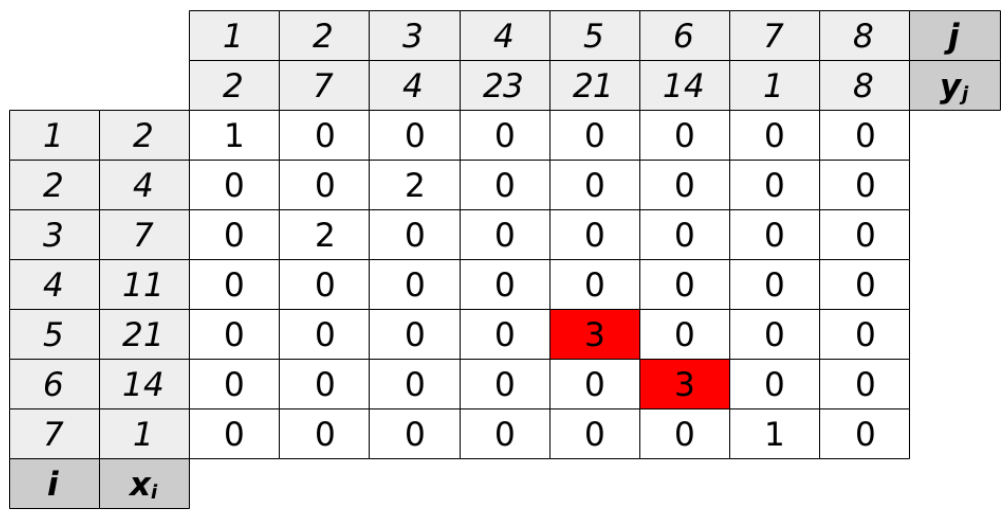
\includegraphics[width = 0.60\linewidth]{Images/9.png}
\end{center}
\begin{algorithm}[H]
    \caption{Algoritmo ricorsivo che risolve un generico sottoproblema $(i,j)$ di LICS}
    \DontPrintSemicolon
    \SetKwFunction{FLICSRic}{LICS-RIC}
    \Proc{\FLICSRic{i,j}} {
        \eIf{$x_I \neq y_j$} {
            \Return 0
        } {
            $max := 0$
            \For{$h \gets 1$ to $i-1$} {
                \For{$k \gets 1$ to $j-1$} {
                    \If{$x_h < x_i$} {
                        $S := $ LICS-RIC$(h,k)$ \;
                        \If{$S > max$} {
                            $max := S$ \;
                        }
                    }
                }
            }
        }
        \Return $1 + max$
    }
\end{algorithm} \noindent
l'algoritmo ricorsivo sopra determina la soluzione $c_{i,j}$
di ogni sottoproblema (si assume di poter accedere alle sequenze $X$ e $Y$).
Questo algoritmo presenta una complessita \textbf{esponenziale}, dato che ogni sottoproblema verrà risolto più volte. Per questa ragione, presentiamo anche un algoritmo scritto
tramite una tecnica bottom-up che permette di calcolare la soluzione di ogni ogni sottoproblema solamente una volta. \newline
\begin{algorithm}[H]
    \caption{Algoritmo iterativo che calcola una LICS tra due sequenze $X$ e $Y$}
    \DontPrintSemicolon
    \SetKwFunction{FLICSIt}{LICS-IT}
    \Proc{\FLICSIt{X,Y}} {
        $max := 0$ \;
        \For{$i \gets 1$ to $m$} {
            \For{$j \gets 1$ to $n$} {
                \eIf{$x_i \neq y_j$} {
                    $c[i,j] := 0$ \;
                    $b[i,j] := (0,0)$ \;
                } {
                    $temp := 0$ \;
                    \For{$h \gets 1$ to $i-1$} {
                        \For{$k \gets 1$ to $j-1$} {
                            \If{$(x_h < x_i) \land (c[h,k] > temp)$ } {
                                $temp := c[h,k]$ \;
                                $b[i,j] := (h,k)$ \;
                            }
                        }
                    }
                    $c[i,j] := 1 + temp$
                }
                \If{$c[i,j] > max$} {
                    $max := c[i,j]$ \;
                    $maxIdx := (i,j)$
                }
            }
        }
        \Return $max$
    }
\end{algorithm} \noindent
\begin{algorithm}[H]
    \caption{Algoritmo di ricostruzione di una LICS tra $X$ e $Y$}
    \DontPrintSemicolon
    \SetKwFunction{FPRINTLICS}{PRINT-LICS}
    \Proc{\FPRINTLICS{i, j, b, c, X}} {
        \eIf{$c[i,j] = 0$} {
            print("non esiste nessuna LCS di $X_i$ e $Y_j$ la quale termini con $x_i = y_j$")
        } {
            \eIf{$b[i,j] \neq (0,0)$} {
                PRINT-LICS($b[i,j]$, b, c, X) \;
                print($x_i$)
            } {
                print($x_i$)
            }
        }
    }
\end{algorithm}
L'algoritmo che calcola una LICS permette di risolvere il problema in tempo:
$$T(n) = \mathcal{O}(m^2 \cdot n^2)$$
occupando $\Theta(m \cdot n)$ spazio in memoria (ossia una matrice che contiene i vari $c_{i,j}$; ovviamente non stiamo contando la matrice $b$).
Si noti che abbiamo utilizzato una matrice $b$ per salvare informazioni utili alla ricostruzione
\begin{center}
    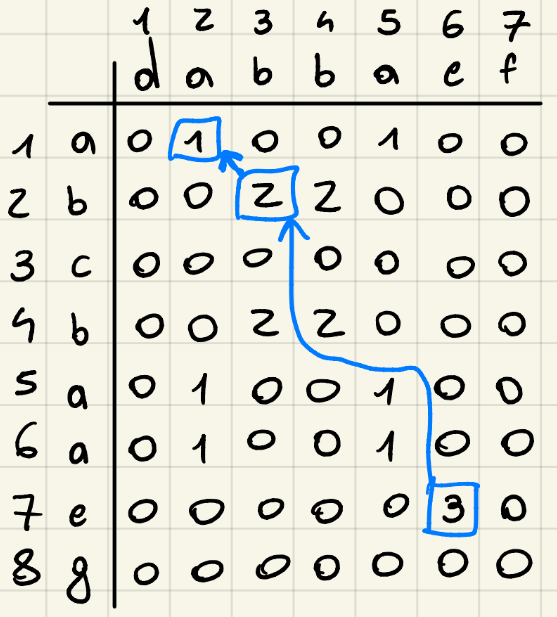
\includegraphics[width = 0.40\linewidth]{Images/10.png}
\end{center}
\subsection{Hateville}
Hateville è una città formata da $n$ case dispose lungo un'unica strada e numerate da $1$ a $n$, in cui si sta organizzando una colletta fondi per la costruzione di un nuovo ospedale.
Ogni abitante $i$ della città è interessato a partecipare e ha già comunicato la quantità di denaro che intende versare, ovvero $d_i$. Ad Hateville però, \textbf{ognuno odia i propri vicini, da entrambi i lati}.
Ovvero, l'abitante della casa $i$ odia i vicini della casa $i-1$ e $i+1$. Per questo motivo, nessuno vuole partecipare ad una colletta a cui partecipano uno o entrambi i propri vicini.
Si vuole quindi determinare \textbf{la massima quantità di denaro che può essere raccolta rispettando questa regola}. \newline
Prima di definire il problema, è necessario introdurre alcune definizioni preliminari.
Sia $X_n = \{1,\dots,n\}$ l'insieme che rappresenta gi $n$ abitanti di Hateville e $A \subseteq X_n$ un suo qualunque sottoinsieme.
Inoltre, sia $(d_1, \dots, d_n)$ un vettore di $n$ elementi con $d_i \in \mathbb{N}$ che rappresenta la quantità di denaro che l'abitante $i$ è disposto a versare.
Possiamo quindi definire il concetto di \textbf{compatibilità} di un sottoinsieme di $X_n$:
\begin{center}
    Un sottoinsieme $A \subseteq X_n$ è \textbf{compatibile} se e solo se $\forall i \in A$ vale che $i-1 \notin A$ e $i+1 \notin A$ (se esistono)
\end{center}
Ovvero, un sottoinsieme $A$ è compatibile se e solo se per nessuno abitante in $A$, $A$ contiene un suo vicino. Possiamo rappresentare questo concetto con la funzione $COMP(A)$:
\begin{center}
    $COMP(A) = True$ se e solo se $\forall i \in A$ vale che $i-1 \notin A$ e $i+1 \notin A$ (se esistono) \\
    $COMP: \mathcal{P}(X_n) \rightarrow \{True, False\}$
\end{center}
Infine, possiamo definire il concetto di \textbf{denaro raccolto} da un sottoinsieme di $X_n$:
\begin{center}
    Il \textbf{denaro raccolto} da un sottoinsieme $A \subseteq X_n$ è la somma delle quantità di denaro che ogni abitante in $A$ è disposto a versare
\end{center}
Ovvero, il denaro raccolto da un sottoinsieme $A$ è la somma dei valori $d_i$ per ogni $i \in A$. Possiamo rappresentare questo concetto con la funzione $D(A)$:
$$D: \mathcal{P}(X_n) \rightarrow \mathbb{R}^+$$
\begin{equation*}
    D(A) = \begin{cases}
        \sum_{i \in A} d_i & \textrm{se } A \neq \emptyset \\
        0 & \textrm{se } A = \emptyset
    \end{cases}
\end{equation*}
Il problema può essere quindi definito come segue: \newline
\textbf{\underline{PROBLEMA}}: Dato $n \in \mathbb{N}$ il numero degli abitanti, rappresentati nell'insieme $X_n = \{1,2,\dots,n\}$ e $d_i, \forall i \in X_n$ la quantità di denaro che l'abitante
$i$ è disposto a versare, determinare un sottoinsieme $S \subseteq X_n$ tale che:
$$COMP(S) = True \land D(S) = \max_{\substack{A \subseteq X_n \\ COMP(A) = True}}\{D(A)\}$$
Il problema può essere formalizzato come segue: \newline
\textbf{\underline{ISTANZA}}: $X_n = \{1,\dots, n\}$ e $d_i, \forall i \in X_n$ \newline
\textbf{\underline{SOLUZIONE}}: $S \subseteq \{1,\dots,n\}$ tale che:
$$COMP(S_n) = True \land D(S_n) = \max_{\substack{A \subseteq X_n \\ COMP(A) = True}}\{D(A)\}$$
Il problema contiene diversi sottoproblemi ognuno dei quali non ha come input l'insieme $X_n$ con $d_i, \forall i \in X_n$ ma un suo sottoinsieme:
\begin{enumerate}
    \item Dato $X_n = \{1,\dots, n\}$, si vuole trovare $S_n \subseteq X_n$ tale che:
    $$COMP(S_n) = True \land D(S_n) = \max_{\substack{A \subseteq X_n \\ COMP(A) = True}}\{D(A)\}$$
    \item Dato $X_{n-1}= \{1,\dots, n-1\}$, si vuole trovare $S_{n-1} \subseteq X_{n-1}$ tale che:
    $$COMP(S_{n-1}) = True \land D(S_{n-1}) = \max_{\substack{A \subseteq X_{n-1}\\ COMP(A) = True}}\{D(A)\}$$
    \item $\dots$
    \item Dato $X_2= \{1,2\}$, si vuole trovare $S_2 \subseteq X_2$ tale che:
    $$COMP(S_2) = True \land D(S_2) = \max_{\substack{A \subseteq X_2\\ COMP(A) = True}}\{D(A)\}$$
    \item Dato $X_1= \{1\}$, si vuole trovare $S_1 \subseteq X_1$ tale che:
    $$COMP(S_1) = True \land D(S_1) = \max_{\substack{A \subseteq X_1\\ COMP(A) = True}}\{D(A)\}$$
    \item Dato $X_0= \emptyset$ si vuole trovare $S_0 \subseteq X_0$ tale che:
    $$COMP(S_0) = True \land D(S_0) = \max_{\substack{A \subseteq X_0\\ COMP(A) = True}}\{D(A)\}$$
\end{enumerate}
Quindi il generico sottoproblema è individuato da $i \in \{0,\dots,n\}$.
Il \textbf{generico sottoproblema di dimensione $i$} è definito come segue: \newline
\textbf{\underline{SOTTOPROBLEMA GENERICO}}: Dato un insieme $X_i = \{1,\dots,i\}$ rappresentante i primi $i$ abitanti di
Hateville, trovare un suo sottoinsieme, che rispetti la compatibilità, che massimizzi il denaro raccolto. \newline
Ossia: \newline
\textbf{\underline{ISTANZA SOTTOPROB. GEN}}: $X_i = \{1,\dots,i\}$ con $d_j, \forall j \in X_i$ \newline
\textbf{\underline{SOLUZIONE SOTTOPROB. GEN}}: $S_i \subseteq \{1,\dots, i\}$ tale che:
$$COMP(S_i) = True \land D(S_i) = \max_{\substack{A \subseteq X_i\\ COMP(A) = True}}\{D(A)\}$$
Dato che $0 \leq i \leq n$ si ottengono $(n+1)$ sottoproblemi, ad ognuno dei quali è associata una \textbf{coppia di variabili}.
Considerato il sottoproblema di dimensione $i$, la coppia di variabili ad esso associata è $(OPT_i, S_I)$ così definita:
\begin{center}
    $OPT_i = D(S_i)$, ossia il valore di un sottoinsieme di $X_i = \{1,\dots,i\}$, che rispetti la compatibilità, che massimizzi il denaro raccolto \\
    $S_i$, un sottoinsieme di $X_i$ che rispetti la compatibilità e che massimizzi il denaro raccolto, pari a $OPT_i$
\end{center}
Per determinare la soluzione di un qualsiasi sottoproblema di dimensione $i$, oltre all'input del problema, si utilizzeranno le soluzioni dei sottoproblemi di dimensione minore.
Si noti che ognuna delle variabili associate ad un sottoproblema è da considerarsi una \textbf{black-box}: si può utilizzare, ma non è possibile conoscerne il contenuto.
Scriviamo le equazioni di ricorrenza: \newline
\textbf{\underline{CASO BASE}}: Se $i = 0 \vee i = 1$ \newline
Il caso base si ha per un qualunque sottoinsieme di dimensione $i$ con $i = 0 \vee i = 1$. Nel caso in cui $i = 0$, il sottoproblema di dimensione $i$ è un
problema \textbf{vuoto}, ossia non ci sono abitanti in Hateville e quindi non c'è nessuno che può partecipare alla colletta.
La soluzione del problema vuoto è quindi $OPT_i = 0$ e $S_i = \emptyset$.
Nel caso in cui $i = 1$ invece, significa che c'è solo un abitante in Hateville e quindi non è necessario fare nessuna scelta per per evitare di inserire i vicini.
La soluzione del sottoproblema di dimensione $i$ considererà quindi solamente l'abitante $1$, di conseguenza $OPT_i = d_1$ e $S_i = \{1\}$. Dunque, il caso base è scrivibile come:
\begin{equation*}
    OPT_i = \begin{cases}
        0 & \textrm{se } i = 0 \\
        d_1 & \textrm{se } i = 1
    \end{cases}
\end{equation*}
\begin{equation*}
    S_i = \begin{cases}
        \emptyset & \textrm{se } i = 0 \\
        \{1\} & \textrm{se } i = 1
    \end{cases}
\end{equation*}
\textbf{\underline{PASSO RICORSIVO}}: Se $i > 1$ \newline
Il passo ricorsivo si ha per un qualunque sottoproblema di dimensione $i$ con $i > 1$, ossia quando ci sono almeno due abitanti in Hateville.
I dati disponibili per calcolare la soluzione del sottoproblema sono: l'input $X_i$ (in particolare la quantità $d_i$) e tutte le soluzioni dei sottoproblemi di dimensione minore.
Per risolvere un sottoproblema, è necessario domandarsi quali sia la struttura di $S_i$ rispetto a $S_{i-1}, \dots, S_0$. Distinguiamo due casi:
\begin{itemize}
    \item Se $i \notin S_i$ allora la soluzione del problema di dimensione $i$ sarà uguale a quella del problema di dimensione $S_{i-1}$; infatti è sufficiente considerare l'insieme di abitanti $\{1,\dots, i-1\}$. Di conseguenza:
    $$OPT_i = OPT_{i-1} \; e \; S_i = S_{i-1}$$
    \item Se $i \in S_i$ allora non è possibile che il vicino $i-1$ partecipi alla colletta, per la regola della compatibilità. Al contrario però, possiamo aggiungere $d_i$ ad $OPT_{i-2}$ e $i$ a $S_{i-2}$ sicuramente senza violare la compatibilità e, dato che $OPT_{i-2}$ era il massimo per il problema
    di dimensione $i-2$, aggiungendo $d_i$ avremo anche il massimo per il problema di dimensione $i$ (se $i \in S_i$). Di conseguenza abbiamo che:
    $$OPT_i = OPT_{i-2} + d_i \; S_i = S_{i-2} \cup \{i\}$$
\end{itemize}
Siccome non possiamo sapere a priori se l'abitante $i$ appartenga o meno alla soluzione, consideriamo entrambe le soluzioni e scegliamo quella di valore massimo.
Formalmente, possiamo scrivere:
$$OPT_i = \max\{OPT_{i-1}, OPT_{i-2} + d_i\}$$
e
\begin{equation*}
    S_i = \begin{cases}
        S_{i-1} & \textrm{se } OPT_{i-1} \geq OPT_{i-2} + d_i \\
        S_{i-2} \cup \{i\} & \textrm{altrimenti}
    \end{cases}
\end{equation*}
\begin{center}
    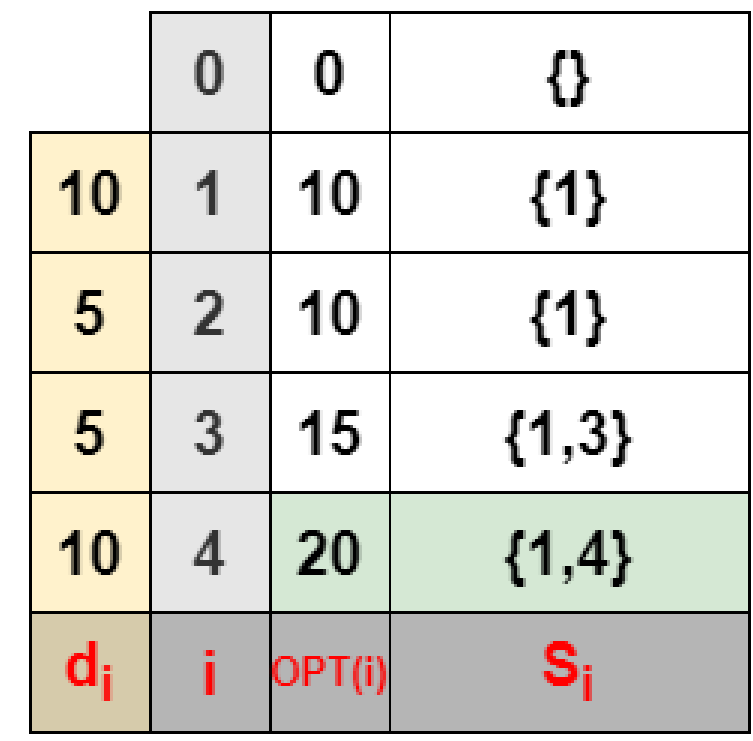
\includegraphics[width = 0.40\linewidth]{Images/11.png}
\end{center}
Una volta calcolati i valori $OPT_0, OPT_1 ,\dots, OPT_n$, è possibile determinare \textbf{la soluzione} al problema andando a considerare
$$(OPT_n, S_n)$$
Enunciamo e dimostriamo il \textbf{teorema della proprietà della sottostruttura ottima}:
\begin{Teorema}[PSO Hateville]
    Sia $i \geq 2$. Siano $S_0, S_1, \dots, S_{i-1}, S_{i-1}$ le soluzioni dei sottoproblemi $0, 1, \dots, i-2, i-1$.
    Sia $S_i$ la soluzione del sottoproblema $i$. Allora:
    \begin{equation*}
        S_i = \begin{cases}
            S_{i-2} \cup \{i\} & \textrm{se } i \in S_i \\
            S_{i-1} & \textrm{se } i \notin S_i
        \end{cases}
    \end{equation*}
\end{Teorema}
\begin{Dimostrazione}
    Distinguiamo i due casi:
    \begin{itemize}
        \item Supponiamo che $i \notin S_i$, devo dimostrare che $S_i = S_{i-1}$. Per assurdo, supponiamo che $S_i \neq S_{i-1}$.
        Allora deve esistere $S' \neq S_{i-1}$ tale che $D(S') > D(S_{i-1})$; inoltre $i \notin S_i$ quindi $S' \subseteq \{1,\dots,i-1\}$, ma così $S_{i-1}$ non
        può più essere soluzione del problema $i-1$-esimo, \textbf{assurdo}!.
        \item Supponiamo che $i \in S_i$, devo dimostrare che $S_i = S_{i-2} \cup \{i\}$. Per assurdo, supponiamo che $S_i \neq S_{i-2} \cup \{i\}$; allora deve esistere $S' \neq S_{i-2} \cup \{i\}$ tale che
        $S'$ è soluzione del problema $i$, quindi tale che $D(S') > D(S_{i-2} \cup \{i\})$; inoltre $S' \subseteq\{1,\dots,i\}$ perché $i \in S_i$ e, inoltre, $COMP(S_i) = True$.
        Infine, $S' = S'' \cup \{i\}$ con $S'' \subseteq\{1,\dots, i-1\}$.
        Quindi:
        $$D(S') > D(S_{i-2} \cup \{i\})$$
        $$D(S'' \cup \{i\}) > D(S_{i-2} \cup \{i\})$$
        $$D(S'') + d_i > D(S_{i-2}) + d_i$$
        $$D(S'') > D(S_{i-2})$$
        Ma quindi $S_{i-2}$ non può più essere soluzione del problema $i-2$; \textbf{assurdo}!.
    \end{itemize}
\end{Dimostrazione}
Utilizzando l'equazione di ricorrenza, possiamo definire un algoritmo ricorsivo che calcoli la soluzione di ogni sottoproblema: \newline
\begin{algorithm}[H]
    \caption{Algoritmo ricorsivo che risolve un generico sottoproblema $i$ di Hateville}
    \DontPrintSemicolon
    \SetKwFunction{FHATEVILLERic}{HATEVILLE-RIC}
    \Proc{\FHATEVILLERic{i}} {
        \eIf{$i = 0$} {
            \Return $(0, \emptyset)$
        } {
            $(V_1, S_1) :=$ HATEVILLE-RIC$(i-1)$ \;
            $(V_2, S_2) :=$ HATEVILLE-RIC$(i-2)$ \;
            $V_2 := V_2 + d_i$ \;
            $S_2 := S_2 \cup \{i\}$ \;
            \eIf{$V_1 \geq V_2$} {
                \Return $(V_1, S_1)$
            } {
                \Return $(V_2, S_2)$
            }
        }
    }
\end{algorithm} \noindent
\newpage \noindent
Questo algoritmo ha \textbf{complessità esponenziale}, visto che ogni sottoproblema viene ricalcolato più volte. Definiamo
quindi un algoritmo bottom-up che calcoli la soluzione al problema: \newline
\begin{algorithm}[H]
    \caption{Algoritmo iterativo che calcola la soluzione al problema Hateville}
    \DontPrintSemicolon
    \SetKwFunction{FHATEVILLEIt}{HATEVILLE-IT}
    \Proc{\FHATEVILLEIt{n}} {
        $OPT[0] := 0$ \;
        $S[0] := \emptyset$ \;
        $OPT[1] := d_1$ \;
        $S[1] := \{1\}$ \;
        \For{$i \gets 1$ to $n$} {
            $V_1 := OPT[i-1]$ \;
            $V_2 := OPT[i-2] + d_i$ \;
            \eIf{$V_1 \geq V_2$} {
                $S[i] := S[i-1]$ \;
                $OPT[i] := V_1$
            } {
                $S[i] := S[i-2] \cup \{i\}$ \;
                $OPT[i] := V_2$
            }
        }
        \Return $(OPT[n], S[n])$
    }
\end{algorithm} \noindent
L'algoritmo ha tempo di esecuzione pari a:
$$T(n) = \mathcal{O}(n)$$
occupando però $\mathcal{O}(n+n^2)$ spazio in memoria (ossia un vettore che contiene i vari $OPT_i$ e un vettore che contiene i vari insiemi $S_i$, ognuno dei quali contiene al massimo $n$ elementi).
Scriviamo l'algoritmo di ricostruzione: \newline
\begin{algorithm}[H]
    \caption{Algoritmo che stampa l'insieme $S_i$ di Hateville}
    \DontPrintSemicolon
    \SetKwFunction{FPRINTHATEVILLE}{PRINT-HATEVILLE}
    \Proc{\FPRINTHATEVILLE{i}} {
        \If{$i \neq 0$} {
            \eIf{$i = 1$} {
                print$(i)$
            } {
                \eIf{$OPT{i-2} + d_i \geq OPT[i-1]$} {
                    PRINT-HATEVILLE$(i-2)$ \;
                    print($i$)
                } {
                    PRINT-HATEVILLE$(i-1)$
                }
            }
        }
    }
\end{algorithm}
\subsection{Distanza di Edit}
Il problema della distanza di edit può essere definito come segue: \newline
\textbf{\underline{PROBLEMA}}: Date due sequenze $X = <x_1, \dots, x_m>$ e $Y = <y_1, \dots, y_n>$, rispettivamente di lunghezza $m$ ed $n$ definite su un alfabeto $\Sigma$, si determini
la \textbf{minima sequenza delle seguenti operazioni elementari} che permette di trasformare $X$ in $Y$ operando una scansione su $X$:
\begin{itemize}
    \item \textbf{insert(a)}: Inserisce $a$ nella posizione corrente della sequenza $X$
    \item \textbf{delete(a)}: cancella $a$ dalla posizione corrente della sequenza $X$
    \item \textbf{replace(a,b)}: sostituisce $a$ con $b$ nella posizione corrente della sequenza $X$
\end{itemize}
Quello che si andrà a risolvere, comunque, è una versione ridotta del problema; la quale è definita come segue: \newline
\textbf{\underline{PROBLEMA RIDOTTO}}: Date due sequenze $X = <x_1,\dots,x_m>$ e $Y = <y_1,\dots,y_n>$, rispettivamente di lunghezza $m$ ed $n$ definite su un alfabeto
$\Sigma$, si determini il \textbf{minimo numero di operazioni elementari} che permette di trasformare $X$ in $Y$ \newline
Il problema ridotto contiene diversi sottoproblemi, ognuno dei quali non ha come input la coppia $(X,Y)$ ma una \textbf{coppia di prefissi di tali sequenze}.
Il sottoproblema generico è quindi individuato dalla coppia $(i,j)$ ed è definito come segue: \newline
\textbf{\underline{SOTTOPROBLEMA GENERICO}}: Date due sequenze $X = <x_1, \dots, x_m>$ e $Y = <y_1, \dots, y_n>$, rispettivamente di lunghezza $m$ ed $n$, si determini il minimo numero di operazioni
elementari che permette di trasformare $X_i$ in $Y_j$. \newline
Dato che $0 \leq i \leq m$ e $0 \leq j \leq n$, si ottengono $(m+1) \cdot (n+1)$ sottoproblemi. Ad ogni sottoproblema \textbf{è associata una variabile}: considerato il sottoproblema di dimensione
$(i,j)$, la variabile ad esso associata è $\delta_{i,j}$ così definita:
\begin{center}
    $d_{i,j} =$ numero minimo di operazioni elementari che permette di trasformare $X_i$ in $Y_j$
\end{center}
Per determinare la soluzione di un qualsiasi sottoproblema $(i,j)$, oltre all'input del problema, si utilizzeranno le soluzioni dei sottoproblemi di dimensione minore.
Scriviamo le \textbf{equazioni di ricorrenza}: \newline
\textbf{\underline{CASO BASE}}: Se $i = 0 \vee j = 0$ \newline
Il caso base si ha per un qualunque sottoproblema di dimensione $(i,j)$ con $i = 0 \vee j = 0$, ossia quando uno dei due prefissi considerati è la sequenza vuota.
In questo cso, è facile ottenere il valore della variabile $\delta_{i,j}$ distinguendo tre casi:
\begin{itemize}
    \item $i = 0 \land j = 0$ allora i prefissi sono entrambi la sequenza vuota; quindi non è necessario alcuna operazione elementare per trasformare $X_i$ in $Y_j$.
    Allora 
    $$\delta_{i,j} = 0$$
    \item $i = 0 \land j > 0$ allora $X_i$ è la sequenza vuota; quindi è necessario eseguire un numero di operazioni elementare pari alla lunghezza del prefisso $Y_j$ (in quanto è necessario inserire tutti gli elementi di $Y_j$ in $X_i$).
    Quindi:
    $$\delta_{i,j} = j$$
    \item $i > 0 \land j = 0$; allora $Y_j$ è la sequenza vuota; quindi è necessario eseguire un numero di operazioni elementari pari alla lunghezza del prefisso $X_i$ (in quanto è necessario eliminare tutti gli elementi di $X_i$). Quindi:
    $$\delta_{i,j} = i$$
\end{itemize}
Il caso base è quindi scrivibile come segue:
\begin{equation*}
    \delta_{i,j} = \begin{cases}
        0 & \textrm{se } i = 0 \land j = 0 \\
        j & \textrm{se } i = 0 \land j > 0 \\
        i & \textrm{se } i > 0 \land j = 0
    \end{cases}
\end{equation*}
\textbf{\underline{PASSO RICORSIVO}}: Se $i > 0 \land j > 0$ \newline
Il passo ricorsivo si ha per un qualunque sottoproblema di dimensione $(i,j)$ con $i > 0 \land j > 0$, ossia quando si vanno a considerare due prefissi
$X_i$ e $Y_j$ entrambi diversi dalla sequenza vuota. I dati disponibili per calcolare $\delta_{i,j}$ sono: l'input $X$ ed in particolare l'elemento $x_i$, l'input $Y$ ed in particolare l'elemento $y_j$ e tutte le variabili $\{\delta_{0,0},\dots, \delta_{i-1, j}, \delta_{i, j-1}\}$.
Per calcolare $\delta_{i,j}$ e quindi risolvere il problema di dimensione $(i,j)$ è necessario distinguere i seguenti casi:
\begin{itemize}
    \item Se $x_i = y_j$; se i due elementi considerati sono identici, allora il numero minimo di operazioni elementari per trasformare $X_i$ in $Y_j$ è uguale al numero minimo di operazioni
    per trasformare il prefisso $X_{i-1}$ in $Y_{j-1}$, ovvero:
    $$\delta_{i,j} = \delta_{i-1, j-1} \; \textrm{se } x_i = y_j$$
    \item Se $x_i \neq y_j$, allora il numero minimo di operazioni è dato dalla soluzione di \textbf{uno dei sottoproblemi di dimensione minore}. Sarà quindi necessario distinguere in base \textbf{all'ultime operazione utilizzata per trasformare $X_i$ in $Y_j$}:
    \begin{itemize}
        \item \textbf{insert($y_j$)}: in questo caso, il numero minimo di operazioni per trasformare $X_i$ in $Y_j$ si ottiene a partire dal numero $\delta_{i,j-1}$ di operazioni per trasformare $X_{i}$ in $Y_{j-1}$ a cui si aggiunge l'operazione di inserimento dell'elemento $y_j$ in $X_i$; ovvero:
        $$\delta_{i,j} = \delta_{i,j-1} + 1$$
        dove 1 rappresenta il contributo dato dall'operazione \textbf{insert($y_j$)}
        \item \textbf{delete($x_i$)}: in questo caso, il numero minimo di operazioni per trasformare $X_i$ in $Y_j$ si ottiene a partire dal numero $\delta_{i-1,j}$ di operazioni per trasformare $X_{i-1}$ in $Y_{j}$ a cui si aggiunge l'operazione di cancellazione dell'elemento $x_i$ da $X_i$; ovvero:
        $$\delta_{i,j} = \delta_{i-1,j} + 1$$
        dove 1 rappresenta il contributo dato dall'operazione \textbf{delete($x_i$)}.
        \item \textbf{replace($x_i$, $y_j$)}: in questo caso, il numero minimo di operazioni per trasformare $X_i$ in $Y_j$ si ottiene a partire dal numero $\delta_{i-1,j-1}$ di operazioni per trasformare $X_{i-1}$ in $Y_{j-1}$ a cui si aggiunge l'operazione di sostituzione dell'elemento $x_i$ con $y_j$ in $X_i$; ovvero:
        $$\delta_{i,j} = \delta_{i-1,j-1} + 1$$
        dove 1 rappresenta il contributo dato dall'operazione \textbf{replace($x_i, y_j$)}.
    \end{itemize}
    Siccome la serie di operazioni \textbf{non è nota}, non possiamo sapere a priori quale dei tre casi si verifichi.
    Quindi consideriamo la soluzione dei tre possibili sottoproblemi e scegliamo quella di valore minimo. Formalmente, possiamo scrivere:
    $$\delta_{i,j} = \min\{\delta_{i, j-1} + 1, \delta_{i-1, j} + 1, \delta_{i-1,j-1} + 1\} \; \textrm{se } x_i \neq y_j$$
\end{itemize}
Il passo ricorsivo è quindi scrivibile come:
\begin{equation*}
    \delta_{i,j} = \begin{cases}
        \delta_{i-1, j-1} & \textrm{se } x_i = y_j \\
        1 + \min\{\delta_{i, j-1} + 1, \delta_{i-1, j} + 1, \delta_{i-1,j-1} + 1\} & \textrm{se } x_i \neq y_j
    \end{cases}
\end{equation*}
\begin{Nota}
    L'equazione di ricorrenza \textbf{è la proprietà della sottostruttura ottima}
\end{Nota}
Una volta calcolati i valori $\delta_{0,0}, \delta_{0,1}, \dots,\delta_{m,n}$ si hanno a disposizione tutte le lunghezze delle sequenze di operazioni per rendere ciascun prefisso $X_i$ uguale al prefisso $Y_j$.
La \textbf{soluzione del problema} è quindi il valore $\delta_{m,n}$.
\begin{center}
    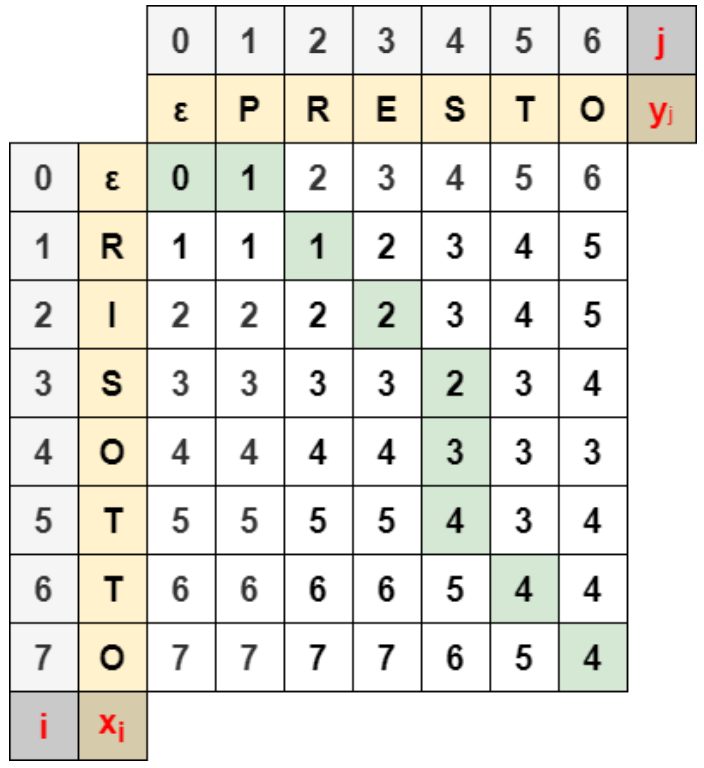
\includegraphics[width = 0.40\linewidth]{Images/12.png}
\end{center}
\begin{algorithm}[H]
    \caption{Algoritmo ricorsivo che calcola la distanza di edit per due prefissi $X_i$ e $Y_j$}
    \DontPrintSemicolon
    \SetKwFunction{FEDRic}{ED-RIC}
    \Proc{\FEDRic{i,j}} {
        \eIf{$i = 0 \vee j = 0$} {
            \eIf{$i = 0$} {
                \Return $j$
            } {
                \Return $i$
            }
        } {
            \eIf{$x_i = y_j$} {
                \Return ED-RIC$(i-1, j-1)$
            } {
                $ins := 1 + \textrm{ED-RIC}(i, j-1)$ \;
                $del := 1 + \textrm{ED-RIC}(i-1, j)$ \;
                $rep := 1 + \textrm{ED-RIC}(i-1, j-1)$ \;
                \Return $MIN(ins, del, rep)$
            }
        }
    }
\end{algorithm} \noindent
L'algoritmo sopra calcola ricorsivamente la soluzione ad un generico sottoproblema $(i,j)$; tuttavia il suo tempo di calcolo è \textbf{esponenziale}.
Scriviamo quindi un algoritmo bottom-up che calcoli la soluzione al problema: \newline
\begin{algorithm}[H]
    \caption{Algoritmo iterativo che calcola la distanza di edit tra due sequenze $X$ e $Y$}
    \DontPrintSemicolon
    \SetKwFunction{FEDIt}{ED-IT}
    \Proc{\FEDIt{X,Y}} {
        \For{$i \gets 0$ to $m$} {
            $\delta[i,0] := i$
        }
        \For{$j \gets 0$ to $n$} {
            $\delta[0, j] := j$
        }
        \For{$i \gets 1$ to $m$} {
            \For{$j \gets 1$ to $n$} {
                \eIf{$x_i = y_j$} {
                    $\delta[i,j] := \delta{i-1, j-1}$
                } {
                    $\delta[i,j] := 1 + MIN(\delta[i,j-1], \delta[i, j-1], \delta[i-1,j-1])$
                }
            }
        }
        \Return $\delta[m,n]$
    }
\end{algorithm} \noindent
L'algoritmo bottom-up ha complessità:
$$T(n) = \mathcal{O}(m \cdot n)$$
e occupa spazio in memoria pari a $\Theta(m \cdot n)$ (ossia una matrice per contenere i vari $\delta_{i,j}$).
\subsection{Varianti di LCS, LIS e LICS}
Presentiamo di seguito, in maniera più o meno formale, delle varianti dei problemi LCS, LIS e LICS.
\subsubsection{LDCS - Longest Decreasing Common Subsequence}
In questa variante di LICS, avviene la seguente variazione all'interno della definizione dell'equazione di ricorrenza:
\begin{itemize}
    \item Se $x_i \neq y_j$ allora
    $$c_{i,j} = 0$$
    \item Se $x_i = y_j$ allora
    $$c_{i,j} = \max\{c_{h,k}|1 \leq h < i \land 1 \leq k < j \land x_h > x_i\} + 1$$
\end{itemize}
la modifica dell'algoritmo bottom-up, per fare in modo che esso rispetti la nuova definizione della variabile $c_{i,j}$, risulta quindi triviale.
\subsubsection{LCS in cui non vi sono due simboli consecutivi che si ripetono}
In questa variante di LCS, vi è la seguente variazione nell'equazione di ricorrenza:
$$c_{i,j} = \max\{c_{h,k}|1 \leq h < i \land 1 \leq k < j \land x_h \neq x_i\} + 1$$
la modifica dell'algoritmo bottom-up, per fare in modo che esso rispetti la nuova definizione della variabile $c_{i,j}$, risulta quindi triviale.
\subsubsection{LCS in cui si alternano numeri pari e numeri dispari}
In questa variante di LCS, vi è la seguente variazione nell'equazione di ricorrenza:
$$c_{i,j} = \max\{c_{h,k}|1 \leq h < i \land 1 \leq k < j \land x_h \bmod 2 \neq x_i \bmod 2\} + 1$$
la modifica dell'algoritmo bottom-up, per fare in modo che esso rispetti la nuova definizione della variabile $c_{i,j}$, risulta quindi triviale.
\subsubsection{LACS - Longest Alternating Common Subsequence}
Sia $C$ un insieme di colori e $col: \Sigma \rightarrow C$ una funzione che attribuisce ad ogni simbolo dell'alfabeto $\Sigma$ un colore.
Possiamo quindi definire così il problema: \newline
\textbf{\underline{PROBLEMA}}: Data due sequenze $X$ e $Y$, rispettivamente di $m$  e $n$ numeri interi, si determini \textbf{\underline{UNA}} tra le più lunghe sottosequenze comuni a $X$ e $Y$ la quale non abbia elementi consecutivi dello stesso colore. \newline
Quello che si andrà a risolvere, comunque, è una versione ridotta del problema, la quale è definita come segue: \newline
\textbf{\underline{PROBLEMA RIDOTTO}}: Date due sequenze $X$ e $Y$, rispettivamente di $m$ ed $n$ numeri interi, si determini \underline{la lunghezza} di una tra le più lunghe sottosequenze comuni a $X$ e $Y$ che non abbia elementi consecutivi dello stesso colore. \newline
Il problema ridotto contiene diversi sottoproblemi ognuno dei quali non ha come input la coppia $(X,Y)$ ma una \textbf{coppia di prefissi} di tali sequenze. Il generico sottoproblema $(i,j)$ è quindi così definito \newline
\textbf{\underline{SOTTOPROBLEMA GENERICO}}: Date due sequenze $X$ e $Y$, rispettivamente di $m$ ed $n$ numeri interi, si determini la lunghezza di una tra le più lunghe sottosequenze comuni a $X_i$ e $Y_j$ la quale non abbia elementi
consecutivi dello stesso colore. \newline
Non consideriamo le coppie $i = 0 \vee j = 0$. Dato che $1 \leq i \leq m$ e $1 \leq j \leq n$, si ottengono $m \cdot n$ sottoproblemi. 
Ad ogni sottoproblema $(i,j)$ è associata \textbf{una variabile} così definita:
\begin{center}
    $c_{i,j} =$ lunghezza di una tra le più lunghe sottosequenze comuni a $X_i$ e $Y_j$ la quale non ha elementi consecutivi dello stesso colore
\end{center}
Per determinare la soluzione di un qualsiasi sottoproblema di dimensione $(i,j)$, oltre all'input del problema, si utilizzeranno le soluzioni dei sottoproblemi di dimensione minore.
Si noti, però, che ogni variabile associata ad un sottoproblema è da considerare come una \textbf{black-box}: si può utilizzare ma non è possibile conoscerne il contenuto.
Il problema così definito \textbf{non è risolvibile poiché ci manca informazione}: date solamente le variabili $\{c_{1,1}, \dots, c_{i-1,j}, c_{i, j-1}\}$ e i prefissi $X_i$ e $Y_j$ (dei quali, in realtà, ci interessano solo gli elementi $x_i$ e $y_j$), non c'è
alcun modo per poter comprendere se gli elementi $x_i$ e $y_j$, nel caso fossero uguali, possano essere accodati alle sottosequenze comuni alternanti relative ai sottoproblemi di dimensione minore a $(i,j)$: non sappiamo \textbf{con quale elemento termini ognuna di queste sottosequenze}, ma ne conosciamo solamente la lunghezza.
Risulta necessario quindi introdurre un \textbf{problema vincolato} nel quale introdurre l'informazione mancante necessaria: \newline
\textbf{\underline{PROBLEMA VINCOLATO}}: Date due sequenze $X$ e $Y$, rispettivamente di $m$ ed $n$ numeri interi, si determini la lunghezza di una tra le più lunghe sottosequenze comuni a $X$ e $Y$ la quale non abbia elementi consecutivi dello stesso colore
e la quale termini con $x_m$ e $y_n$ (se questi coincidono, $0$ in caso contrario). \newline
Come per il problema ridotto, anche il problema vincolato contiene $m \cdot n$ diversi sottoproblemi, ognuno \textbf{associato ad una differente variabile}. Il sottoproblema generico del problema vincolato di dimensione $(i,j)$ è definito come segue: \newline
\textbf{\underline{SOTTOPROB. GEN. PROBL. VINCOLATO}}: Date due sequenze $X$ e $Y$, rispettivamente di $m$ ed $n$ numeri interi, si determini la lunghezza di una tra le più lunghe sottosequenze comuni a $X_i$ e $Y_j$ la quale non abbia elementi consecutivi dello stesso colore
e la quale termini con $x_i$ e $y_j$ (se questi coincidono, $0$ in caso contrario). \newline
il sottoproblema è associato alla variabile $c_{i,j}$ così definita:
\begin{center}
    $c_{i,j} =$ lunghezza di una tra le più lunghe sottosequenze comuni a $X_i$ e $Y_j$ la quale non ha elementi consecutivi dello stesso colore e la quale termina con $x_i$ e $y_j$ (se questi coincidono)
\end{center}
Si noti quindi che per un qualunque sottoproblema di dimensione $(s,t)$, solo imponendo che la soluzione $c_{s,t}$ si riferisca ad una sottosequenza comune a $X_s$ e $Y_t$ la quale non presenta elementi consecutivi dello stesso colore e la quale termina con $x_s = y_t$ è possibile stabilire se un altro elemento $x_u = y_v$ con $u >s$ e $v>t$ possa essere accodato a tale sottosequenza (andando a verificare che 
$col(x_s) = col(y_t) \neq col(x_u) = col(y_v)$).
Scriviamo le \textbf{equazioni di ricorrenza}: \newline
\textbf{\underline{CASO BASE}}: $(i,j)$ con $i > 0 \land j > 0$ tali che $x_i \neq y_j$ \newline
Certamente fanno parte del caso base tutte le coppie $(i,j)$ tali che $x_i \neq y_j$, ossia quando i due prefissi $X_i$ e $Y_j$ terminano con due elementi diversi.
Questo caso, infatti, è semplice da risolvere: per definizione di $c_{i,j}$, gli elementi $x_i$ e $y_j$ devono coincidere, in caso contrario la soluzione è $0$ (ossia non c'è nessuna soluzione).
Il numero di sottoproblemi che compone il problema vincolato possono essere ridotti a $m \cdot n$. Allora $c_{i,j}$ è scrivibile come:
$$c_{i,j} = 0$$
\textbf{\underline{PASSO RICORSIVO}}: $(i,j)$ con $i > 0 \land j > 0$ tali che $x_i = y_j$ \newline
Il passo ricorsivo si ha per un qualunque sottoproblema di dimensione $(i,j)$ tale che $x_i = y_j$, ossia quando i due prefissi $X_i$ e $Y_j$ considerati terminano con lo stesso elemento.
In questo caso, la lunghezza della più lunga sottosequenza con colori alternanti comune fra $X_i$ e $Y_j$ è uguale alla lunghezza della più lunga sottosequenza comune con colori alternanti calcolata per un sottoproblema di dimensione minore e che termina con un carattere con colore diverso da quello di $x_i = y_j$ aumentata di uno.
Il tutto può essere scritto come:
$$c_{i,j} = 1 + \max\{c_{h,k}|1 \leq h < i, 1 \leq k < j, col(x_i) \neq col(x_h)\}$$
Poiché può accadere che l'insieme $\{c_{h,k}|1 \leq h < i, 1 \leq k < j, col(x_i) \neq col(x_h)\}$ sia vuoto (il che corrisponde al fatto che l'elemento $x_i = y_j$ è colorato allo stesso modo di tutti gli elementi precedenti e, quindi, non può essere accodato a nessuna più lunga sottosequenza alternante relativa a sottoproblemi di dimensione minore),
assumiamo per definizione che $\max \emptyset = 0$, così che il corrispondente valore di $c_{i,j}$ risulti uguale a $1$. Inoltre, si noti che l'insieme $\{c_{h,k}|1 \leq h < i, 1 \leq k < j, col(x_i) \neq col(x_h)\}$ corrisponde all'insieme vuoto anche se $i = 1 \vee j = 1$, in quanto i casi $i = 0 \vee j = 0$ non sono considerati e, pertanto, non esistono
sottoproblemi di dimensione minore a quella del sottoproblema considerato. \newline
Una volta calcolati i valori $c_{1,1}, c_{2,1}, \dots, c_{m,n}$, si hanno a disposizione tutte le lunghezze delle sottosequenze comuni massimali fra qualsiasi prefisso di $X$ e qualsiasi prefisso di $Y$ le quali non hanno elementi consecutivi dello stesso colore e le quali terminano con l'ultimo elemento di entrami i prefissi.
La \textbf{soluzione al problema vincolato} è $c_{m,n}$ mentre la \textbf{soluzione al problema ridotto} è:
$$\max\{c_{i,j}|1 \leq i \leq m \land 1 \leq j \leq n\}$$
\begin{center}
    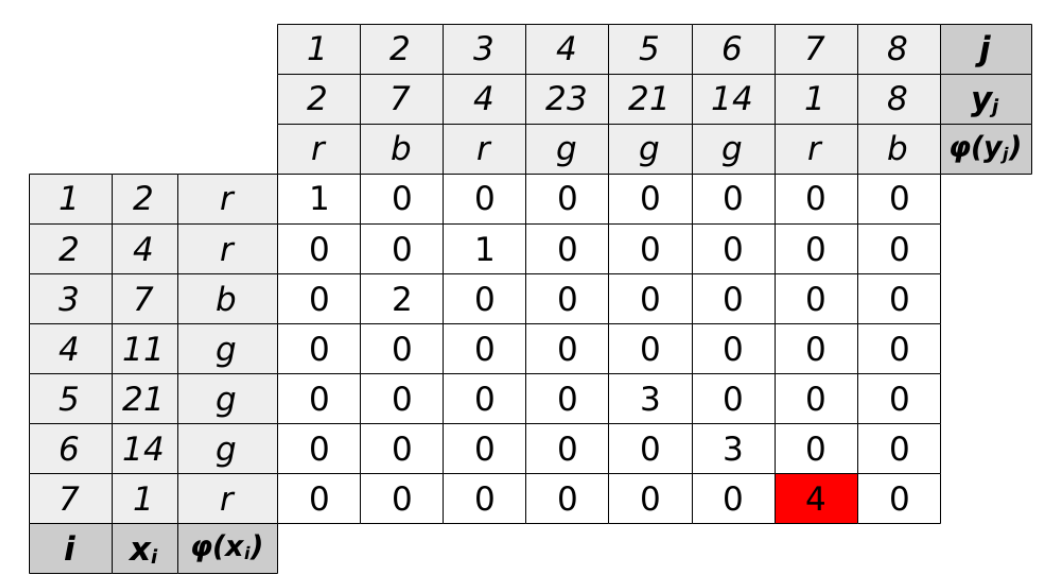
\includegraphics[width = 0.60\linewidth]{Images/13.png}
\end{center}
Utilizzando le equazioni di ricorrenza, scriviamo un algoritmo ricorsivo che calcola la soluzione ad un generico sottoproblema $(i,j)$: \newline
\begin{algorithm}[H]
    \caption{Algoritmo ricorsivo che calcola la soluzione ad un gen. sottoprob. $(i,j)$ di LACS}
    \DontPrintSemicolon
    \SetKwFunction{FLACSRic}{LACS-RIC}
    \Proc{\FLACSRic{i, j}} {
        \eIf{$x_i \neq y_j$} {
            \Return 0
        } {
            $max := 0$ \;
            \For{$h \gets 1$ to $i-1$} {
                \For{$k \gets 1$ to $j-1$} {
                    \If{$col(x_h) \neq col(x_i)$} {
                        $S :=$ LACS-RIC$(h,k)$ \;
                        \If{$S > max$} {
                            $max := S$
                        }
                    }
                }
            }
        }
        \Return $1 + max$
    }
\end{algorithm} \noindent
l'algoritmo sopra ha \textbf{complessità esponenziale}; scriviamo quindi un algoritmo bottom-up che calcoli la soluzione al problema: \newline
\begin{algorithm}[H]
    \caption{Algoritmo bottom-up che calcola la soluzione al problema LACS}
    \DontPrintSemicolon
    \SetKwFunction{FLACSIt}{LACS-IT}
    \Proc{\FLACSIt{X,Y}} {
        $max := 0$ \;
        \For{$i \gets 1$ to $m$} {
            \For{$j \gets 1$ to $n$} {
                \eIf{$x_i \neq y_j$} {
                    $c[i,j] := 0$
                } {
                    $temp := 0$ \;
                    \For{$h \gets 1$ to $i-1$} {
                        \For{$k \gets 1$ to $j-1$} {
                            \If{$(col(x_h) \neq col(x_i)) \land (c[h,k] > temp)$} {
                                $temp := c[h,k]$
                            }
                        }
                    }
                    $c[i,j] := 1 + temp$ \;
                }
                \If{$c[i,j] > max$} {
                        $max := c[i,j]$
                    }
            }
        }
        \Return $max$
    }
\end{algorithm} \noindent
L'algoritmo ha complessità computazionale pari a:
$$T(n) = \mathcal{O}(m^2 \cdot n^2)$$
e occupa uno spazio pari a $\Theta(m \cdot n)$ (ossia una matrice che contiene i vari $c_{i,j}$).
\subsubsection{LCS senza due pari consecutivi}
In questa variante di LCS, vi è la seguente variazione alla definizione della variabile:
$$c_{i,j} = \max\{c_{h,k}|1 \leq h < i \land 1 \leq k < j \land x_h \bmod 2 \neq 0 \land x_i \bmod 2 \neq 0\} + 1$$
la modifica dell'algoritmo bottom-up, per fare in modo che esso rispetti la nuova definizione della variabile $c_{i,j}$, risulta quindi triviale.
\subsubsection{LCSR: LCS con al massimo R simboli rossi}
\textbf{\underline{ISTANZA}}: $X_m$ e $Y_n$ sequenze \newline
\textbf{\underline{SOLUZIONE}}: Calcolare \underline{la lunghezza} di una più lunga sottosequenza di $X_m$ e $Y_n$ la quale ha al massimo $R$ simboli colorati di rosso. \newline
Si assume di avere una funzione $col: \Sigma \rightarrow \{Red, Blue\}$ e che ad ogni simbolo all'interno delle due sequenze ha un colore che è il rosso oppure il blu. \newline
Ogni \textbf{sottoproblema generico} è quindi \textbf{identificato da una tripla} $(i, j, r)$ con:
$$i \in \{0,\dots, m\}$$
$$j \in \{0,\dots, m\}$$
$$r \in \{0\dots, R\}$$
ad ogni sottoproblema è \textbf{associata una variabile} così definita:
\begin{center}
    $c_{i,j,r} =$ la lunghezza di una più lunga sottosequenza comune di $X_i$ e $Y_j$ con $r$ simboli rossi
\end{center}
Definiamo le \textbf{equazioni di ricorrenza}: \newline
\textbf{\underline{CASO BASE}}: $(i,j,r)$ con $i = 0 \vee j = 0, \forall r \in \{0,\dots,R\}$ \newline  
In questo caso, una (o entrambe) le sottosequenze sono \textbf{vuote}, quindi la lunghezza di una più lunga sottosequenza comune a $X_i$ e $Y_j$ con $r$ simboli rossi è:
$$c_{i,j,r} = 0$$
\textbf{\underline{PASSO RICORSIVO}}: $(i,j,r)$ con $i > 0 \land j > 0$ e con $r$ qualsiasi \newline
Visto che $i > 0 \land j > 0$, allora entrambe i prefissi considerati \textbf{non sono la sequenza vuota}. Dobbiamo distinguere due casi:
\begin{itemize}
    \item Se $x_i \neq y_j$ allora significa che dobbiamo prendere il valore massimo tra i due problemi di dimensione $(i-1, j, r)$ e $(i, j-1, r)$; quindi la variabile avrà valore
    $$c_{i, j, r} = \max\{c_{i-1, j, r}, c_{i, j-1, r}\}$$
    \item Se $x_i = y_j$ allora significa che $x_i = y_j$ potrebbe appartenere alla sottosequenza soluzione del problema. Dobbiamo quindi distinguere altri due sotto-casi:
    \begin{itemize}
        \item Se $col(x_i) = Red$ allora dobbiamo stare attenti a \textbf{quanti simboli rossi sono già presenti all'interno della sottosequenza}
        \begin{itemize}
            \item Se $r = 0$ allora $$c_{i,j,r} = c_{i-1, j-1, 0}$$
            cioè \textbf{non posso aggiungere il simbolo $x_i$} poiché "non c'è più spazio" per ulteriori simboli rossi
            \item Se $0 < r \leq R$ allora $$c_{i, j, r} = c_{i-1, j-1, r-1} + 1$$
        \end{itemize}
        \item Se $col(x_i) \neq Red$ allora
        $$c_{i,j,r} = c_{i-1, j-1, r} +1$$
    \end{itemize}
\end{itemize}
Il passo ricorsivo è quindi riassumibile come segue:
\begin{equation*}
    c_{i,j,r} = \begin{cases}
        \max\{c_{i-1, j, r}, c_{i, j-1, r}\} & \textrm{se } x_i \neq y_j \\
        \begin{cases}
            \begin{cases}
                c_{i-1, j-1, 0} & \textrm{se } $r = 0$ \\
                c_{i-1, j-1, r} + 1 & \textrm{se } 0 < r \leq R
            \end{cases} & \textrm{se } col(x_i) = Red \\
            c_{i-1, j-1, r} + 1 & \textrm{se } col(x_i) \neq Red
        \end{cases} & \textrm{se } x_i = y_j
    \end{cases}
\end{equation*}
Scriviamo quindi l'algoritmo bottom-up per calcolare la soluzione al problema \newline
\begin{algorithm}[H]
    \caption{Algoritmo iterativo che calcola al soluzione al problema LCSR}
    \DontPrintSemicolon
    \SetKwFunction{FLCSRit}{LCSR-IT}
    \Proc{\FLCSRit{X,Y,R}} {
        $m := LENGTH(X)$ \;
        $n := LENGTH(Y)$ \;
        \For{$i \gets 0$ to $m$} {
            \For{$r \gets 0$ to $R$} {
                $c[i, 0, r] := 0$
            }
        }
        \For{$j \gets 0$ to $n$} {
            \For{$r \gets 0$ to $R$} {
                $c[0, j, r] := 0$
            }
        }
        \For{$i \gets 1$ to $m$} {
            \For{$j \gets 1$ to $n$} {
                \For{$r \gets 0$ to $R$} {
                    \eIf{$x_i \neq y_j$} {
                        $c[i,j,r] := \max\{c[i-1,j,r], c[i, j-1, r]\}$
                    } {
                        \eIf{$col(x_i) \neq Red$} {
                            $c[i,j,r] := c[i-1,j-1,r] + 1$
                        } {
                            \eIf{$r = 0$} {
                                $c[i,j,r] := c[i-1,j-1,0]$
                            } {
                                $c[i,j,r] := c[i-1,j-1, r-1] +1$
                            }
                        }
                    }
                }
            }
        }
        \Return $c[m, n, R]$
    }
\end{algorithm} \noindent
l'algoritmo ha complessità computazionale pari a:
$$T(n) = \Theta(m \cdot n \cdot R)$$
\newpage \noindent
Presentiamo inoltre l'algoritmo di ricostruzione: \newline
\begin{algorithm}[H]
    \caption{Algoritmo che stampa la soluzione al problema LCSR}
    \DontPrintSemicolon
    \SetKwFunction{FPRINTLCSR}{PRINT-LCSR}
    \Proc{\FPRINTLCSR{X,Y,i,j,r}} {
        \If{$i \neq 0 \land j \neq 0$} {
            \eIf{$x_i \neq y_j$} {
                \eIf{$c[i-1,j,r] \geq c[i,j-1,r]$} {
                    PRINT-LCSR(X, Y, i-1, j, r)
                } {
                    PRINT-LCSR(X, Y, i, j-1, r)
                }
            } {
                \eIf{$col(x_i) \neq Red$} {
                    PRINT-LCSR(X, Y, i-1, j-1, r) \;
                    print($x_i$)
                } {
                    \eIf{$r = 0$} {
                        PRINT-LCSR(X,Y, i-1, j-1, 0)
                    } {
                        PRINT-LCSR(X, Y, i-1, j-1, r-1) \;
                        print($x_i$)
                    }
                }
            }
        }
    }
\end{algorithm} \noindent
\subsubsection{Stabilire se tutte le LCS di X e Y hanno almeno R simboli rossi}
Siano $X$ e $Y$ due sequenze, rispettivamente di $m$ ed $n$ simboli, costruite sull'alfabeto $\Sigma$ e sia $col$ la funzione:
$$col: \Sigma \rightarrow \{Red, Blue\}$$
Il problema è quindi così definito: \newline
\textbf{\underline{PROBLEMA}}: Stabilire se tutte le LCS di $X$ ed $Y$ hanno almeno $R$ simboli rossi \newline
Ogni sottoproblema generico è individuato da una tripla $(i,j,r)$ con $r \in \{0,\dots, R\}$ ed è così definito \newline
\textbf{\underline{SOTTOPROBLEMA GENERICO}}: Stabilire se tutte le LCS di $X_i$ e $Y_j$ hanno almeno $R$ simboli rossi. \newline
Ad ogni sottoproblema è \textbf{associata una variabile} così definita:
\begin{equation*}
    e_{i,j,r} = \begin{cases}
        True & \textrm{Se tutte le LCS di } X_i \; e \; Y_j \; \textrm{hanno almeno } R \; \textrm{simboli rossi} \\
        False & \textrm{Altrimenti}
    \end{cases}
\end{equation*}
Scriviamo \textbf{l'equazione di ricorrenza}: \newline
\textbf{\underline{CASO BASE}}: $(i,j,r)$ con $(i = 0 \vee j = 0)$ e $\forall r \in \{0,\dots, R\}$ \newline
In questo caso, abbiamo che:
\begin{equation*}
    e_{i,j,r} = \begin{cases}
        True & \textrm{se } r = 0 \\
        False & \textrm{se } r > 0
    \end{cases}
\end{equation*}
\textbf{\underline{PASSO RICORSIVO}}: $(i,j,r)$ con $i > 0 \land j > 0$ e $\forall r \in \{0,\dots,R\}$ \newline
Assumiamo di aver \textbf{già calcolato le lunghezze di tutte le LCS tra $X_i$ e $Y_j$} e di averle salvate nelle variabili $c_{i,j}$ (asintoticamente, questo non modifica i tempi dell'algoritmo).
Dobbiamo in questo caso distinguere diversi casi:
\begin{itemize}
    \item Se $x_i \neq y_j$ allora:
    \begin{center}
        $e_{i,j,r} = \begin{cases}
            e_{i-1, j, r} & \textrm{Se } c_{i-1, j} > c_{i, j-1} \\
            e_{i, j-1, r} & \textrm{Se } c_{i, j-1} > c_{i-1, j} \\
            e_{i-1,j,r} \land e_{i, j-1, r} & \textrm{Se } c_{i-1,j} = c_{i, j-1}
        \end{cases}$
    \end{center}
    \item Se $x_i = y_j$ dobbiamo distinguere altri 3 sotto-casi:
    \begin{itemize}
        \item Se $col(x_i) \neq Red$ allora:
        $$e_{i,j,r} = c_{i-1, j-1, r}$$
        \item Se $col(x_i) = Red \land r > 0$ allora:
        $$e_{i,j,r} = c_{i-1, j-1, r-1}$$
        \item Se $col(x_i) = Red \land r = 0$ allora:
        $$e_{i,j,r} = c_{i-1, j-1, 0} = True$$  
    \end{itemize}
\end{itemize}
La \textbf{soluzione al problema} sarà in $e_{m,n,R}$.
\subsubsection{Stabilire se tutte le LCS di X ed Y hanno numero pari di simboli rossi}
Assumiamo di essere nella stessa situazione del paragrafo precedente per quanto riguarda $X$, $Y$ e $col$.
Il problema è quindi così definito: \newline
\textbf{\underline{PROBLEMA}}: Stabilire se tutte le LCS di $X$ e $Y$ hanno un numero pari di simboli rossi. \newline
Ogni sottoproblema è individuato da una tripla $(i,j,p)$ con $p = 0$ che indica che il sottoproblema ha \textbf{un numero pari di simboli rossi}
e $p = 1$ che indica l'opposto. Ad ogni sottoproblema è associata \textbf{una variabile} così definita:
\begin{equation*}
    e_{i,j,p} = \begin{cases}
        True & \textrm{Se } p = 0 \\
        False & \textrm{Se } p = 1
    \end{cases}
\end{equation*}






\end{document}
